\documentclass[11pt]{report}
\usepackage[english]{babel}
\usepackage{natbib}
\usepackage{url}
\usepackage[utf8x]{inputenc}
\usepackage{amsmath}
\usepackage{graphicx}
\graphicspath{{images/}}
\usepackage{parskip}
\usepackage{fancyhdr}
\usepackage{vmargin}
\usepackage{colortbl}
\usepackage{hyperref}
\setmarginsrb{3 cm}{2.5 cm}{3 cm}{2.5 cm}{1 cm}{1.5 cm}{1 cm}{1.5 cm}

\author{SOW Sokhna Maimouna} % Author

\makeatletter
\let\theauthor\@author
\renewcommand{\thesection}{\@arabic\c@section}


\makeatother

\pagestyle{fancy}
\fancyhf{}
\lhead{\theauthor}
\rhead{\rightmark}
\lfoot{Universite Paris Ouest}
\rfoot{Cosmo Consult}
\cfoot{\thepage}
\renewcommand{\footrulewidth}{0.4pt}%trait horizontal pour le pied de page

\begin{document}

%%%%%%%%%%%%%%%%%%%%%%%%%%%%%%%%%%%%%%%%%%%%%%%%%%%%%%%%%%%%%%%%%%%%%%%%%%%%%%%%%%%%%%%%%

\begin{titlepage}

\includegraphics[scale=0.5]{images/image1.jpg} \hspace*{\stretch{1}}

\includegraphics[scale=0.3]{images/image2.png}
\vspace*{\stretch{4}}

\hrulefill
\begin{center}\bfseries\huge
     RAPPORT DE STAGE
\end{center}

\begin{center}\bfseries\Huge
	Project Assistant
\end{center}

\begin{center}\bfseries\huge
Mise en place d'un outil d'agrégation de calendrier et de planification
\end{center}
\hrulefill

\vspace*{4cm}
\textbf{SOW Sokhna Maimouna} \hspace*{\stretch{1}} 
Enseignant Tuteur : \textbf{Marta Rukoz} \\
M1 MIAGE Classique \hspace*{\stretch{1}}
Maître de stage : \textbf{Xavier Garonnat} \\
Année 2016/2017 \\ 
 
\end{titlepage}

%page de garde
\thispagestyle{empty}
\newpage
~

\newpage
\section{Remerciements}
\hspace{1cm} Je tiens tout d’abord à remercier mon tuteur de stage, \textbf{Monsieur Xavier Garonnat}, pour sa disponibilité et son assistance, malgré le peu de temps qu’il a. Il est très attentif et compréhensif. Ses explications et ses conseils à la recherche de solutions meilleures m’ont beaucoup aidée à trouver le chemin adéquate.\\ 

\hspace{1cm} Mes remerciements s’adressent également à mon maître de stage \textbf{Madame Marta Rukoz} pour son attention envers moi et pour sa disponibilité, à mon responsable de formation \textbf{Monsieur Pascal Poizat} pour ses conseils durant toute l’année scolaire et tout le \textbf{corps professionnel} de l’université Paris Nanterre.\\ 

\hspace{1cm} Je remercie également \textbf{Monsieur Jean-Marc Garel} pour sa confiance et toute son aide. Mes remerciements s’adressent également à toute l’équipe de Cosmo Consult particulièrement à \textbf{Monsieur Christophe Reulier} qui m’a bien accueillie à bras ouvert et m’a beaucoup aidé à m’intégrer dans l’entreprise.\\

\hspace{1cm} Et enfin je dis un grand merci à \textbf{ma grande sœur} qui m’a toujours soutenue et aidée dans mes études, à mes parents et à tous mes proches.


%%%%%%%%%%%%%%%%%%%%%%%%%%%%%%%%%%%%%%%%%%%%%%%%%%%%%%%%%%%%%%%%%%%%%%%%%%%%%%%%%%%%%%%%%
\newpage
\renewcommand{\contentsname}{Table des matières}
\tableofcontents
\pagebreak

%%%%%%%%%%%%%%%%%%%%%%%%%%%%%%%%%%%%%%%%%%%%%%%%%%%%%%%%%%%%%%%%%%%%%%%%%%%%%%%%%%%%%%%%%

\section{Introduction}
\hspace{1cm} Dans le cadre de l'obtention du diplôme de M1 MIAGE, nous sommes appelés à effectuer un stage obligatoire de 3 mois minimum. Ce stage nous permettra de mettre en pratique les enseignements théoriques de la formation à savoir la gestion de projet et/ou le développement informatique et de nous familialiser au monde professionnel.\\
 
\hspace{1cm} J'ai eu la chance d'être accueillie comme stagiaire chez Cosmo Consult, du 03 avril au 14 août 2017. Ayant déjà fait un stage en tant que développeur, j'ai saisi l'opportunité d'être dans une formation à double compétence pour me lancer, cette année dans ce stage comme assistante de projet.\\ 
 
\hspace{1cm} Dans un premier temps je vous présenterai l'entreprise, son historique, sa structuration et ses activités. Ensuite j'aborderai le déroulement de mon stage, mes principales missions au sein de Cosmo Consult France avec les méthodes adoptées pour mener à bout ce qui m'a été confiée et les problèmes rencontrés. Et pour finir je ferais un bilan pour exprimer ce que ce stage m'a apportée.

\newpage
\section{Cosmo Consult}
	\subsection{Présentation du groupe}
\hspace{1cm} Cosmo Consult International a été créé en 1996. C'est une société européenne indépendante, présente en Allemagne, Espagne, Suède et France, et qui est devenue l'un des leaders européens de l’intégration des solutions Microsoft Dynamics et éditeur de logiciels métiers basés sur les technologies Microsoft.  Cosmo accompagne ses clients, PME/PMI et filiales de grands groupes dans leurs projets de transformation numérique et d’évolution de leur Système d’Information.\\

\hspace{1cm} De nos jours elle compte près de 650 collaborateurs répartis sur 20 succursales en Europe et plus de 2000 clients dans le monde entier. Elle est dans le top 3 de l'intégration Dynamics en Europe et dans le top 5 des partenaires Dynamics dans le monde. Elle a une performance durable et soutenue avec un chiffre d'affaire de près de 19 millions d'euros en 2012 et 90 millions d'euros en 2016. 

	\subsection{Présentation de Cosmo Consult France}
\hspace{1cm} La France rejoint le groupe en juin 2015. Cosmo Consult France est une filiale en pleine expansion avec un plan de développement ambitieux sur les 3 prochaines années. Elle est partenaire stratégique Microsoft avec une équipe Dynamics NAV expérimentée dans :
\begin{itemize}
	\item L’intégration :
		\begin{itemize}
			\item L’implémentation ERP
			\item Business Intelligence
			\item Content Management
		\end{itemize}
		
	\item L’évolution du SI :
		\begin{itemize}
			\item Optimisation
			\item Migration
		\end{itemize}	 
	\item Le support  
	\item L'éditeur de solution métiers
\end{itemize}

\hspace{1cm} Cosmo Consult est devenue l'un des plus grands fournisseurs de logiciels sectoriels et de gestion pour les PME et les grandes entreprises, basés sur les dernières technologies Microsoft et QlikView.\\

	\subsection{L'organisation de Cosmo Consult}
\hspace{1cm}L'équipe Cosmo Consult France est composée d'une direction des opérations et d'une direction commerciale. Au sein de ces deux directions, nous retrouvons des chefs de projets, des responsables marketing, des développeurs, des chefs d'équipe de soutien, des hauts comptables des consultants fonctionnels et des consultants séniors.\\

Ci-dessous l'organigramme de toute l'équipe Cosmo Consult France.
\begin{center}
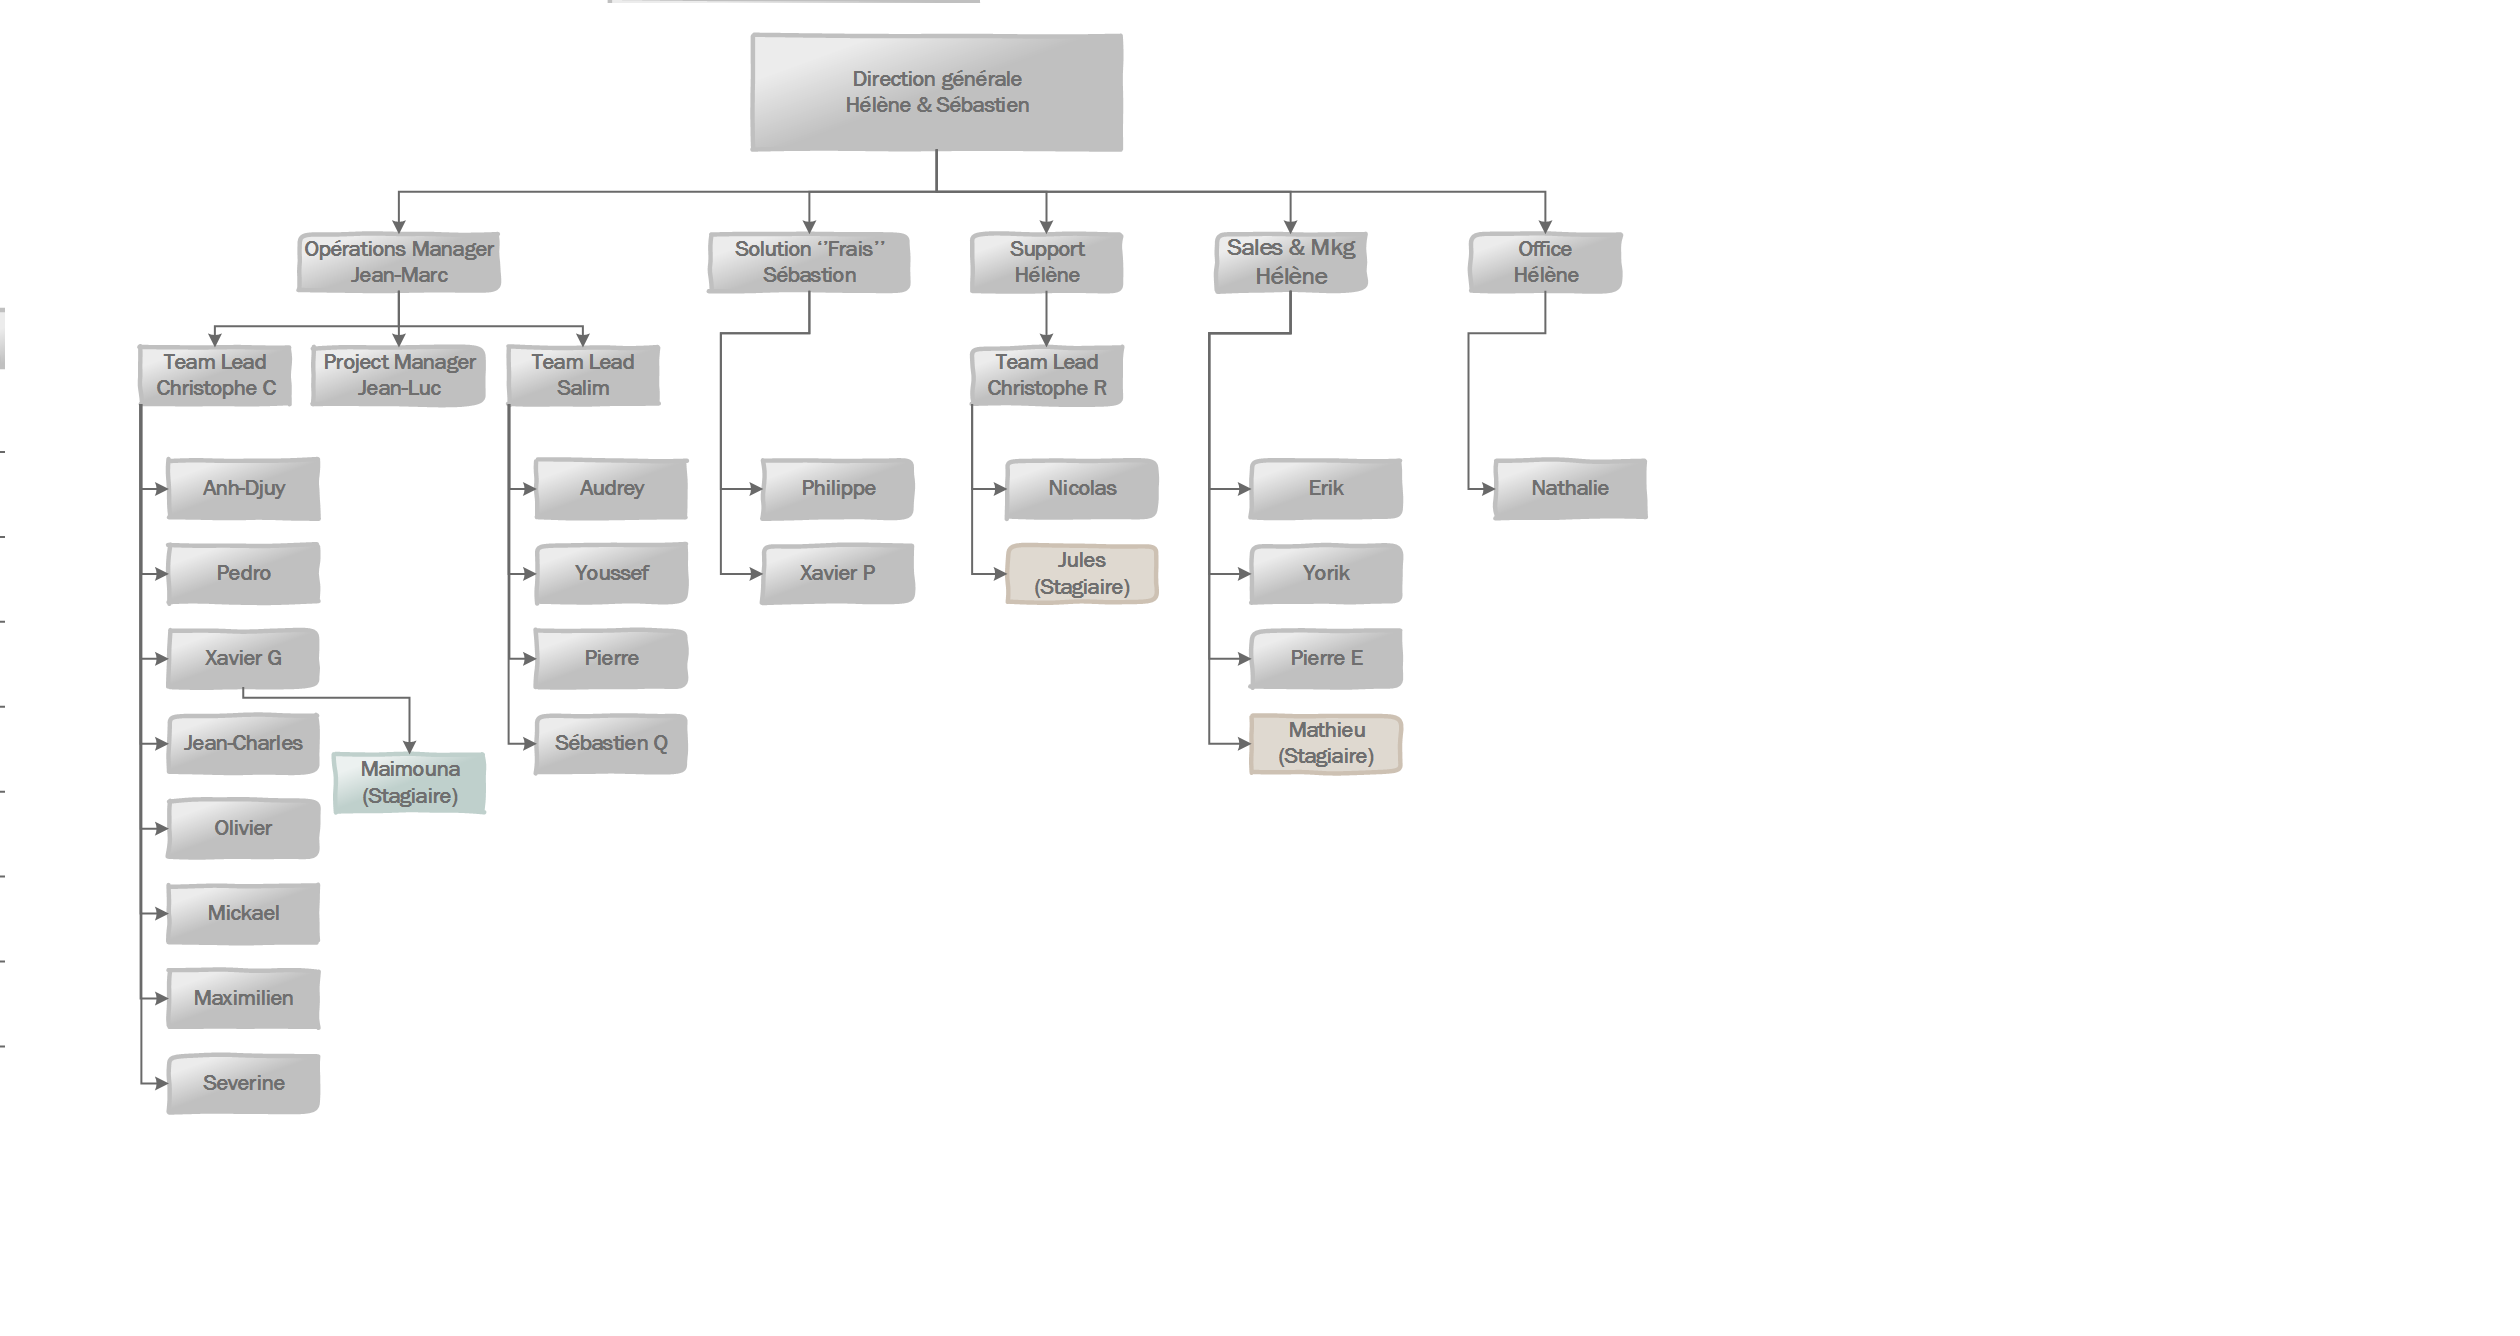
\includegraphics[scale=0.5]{images/figure1.png}
\vspace*{\stretch{-10}}
\underline{\textbf{Figure 1 : Organigramme de Cosmo}}
\end{center}

	\subsection{Les activités de Cosmo Consult France}
\hspace{1cm} Cosmo Consult France est devenu le leader en France sur le marché des solutions Dynamics et des services de conseil et d'intégration auprès de sociétés nationales et internationales. Cosmo Consult France offre les solutions : 
\begin{itemize}
	\item\textbf{ ERP Gestion à l'affaire} : pour les équipements industriels, producteurs d'équipements spéciaux, les sociétés de services, de conseil et d'ingénierie, les bureaux d'études…
	
	\item \textbf{ERP Discrete Manufacturing} : pour la fabrication d'équipements spécifiques ou configurables, en petite séries ou à la commande, le service après-vente, les modes de gestion engineer-to-order, make-to-order…
	
	\item \textbf{ERP Process Manufacturing} : pour les secteurs de la plasturgie, de la chimie fine, de l'industrie du verre et de la céramique, des colles, vernis, peintures…
	
	\item \textbf{ERP Life Sciences} : pour les secteurs de la pharmacie, des biotechnologies, des compléments alimentaires, de la cosmétique et les fabricants d'équipements médicaux…
\end{itemize}

Nous pouvons constater sur la figure suivante certains de nos clients par secteur : 
\begin{center}
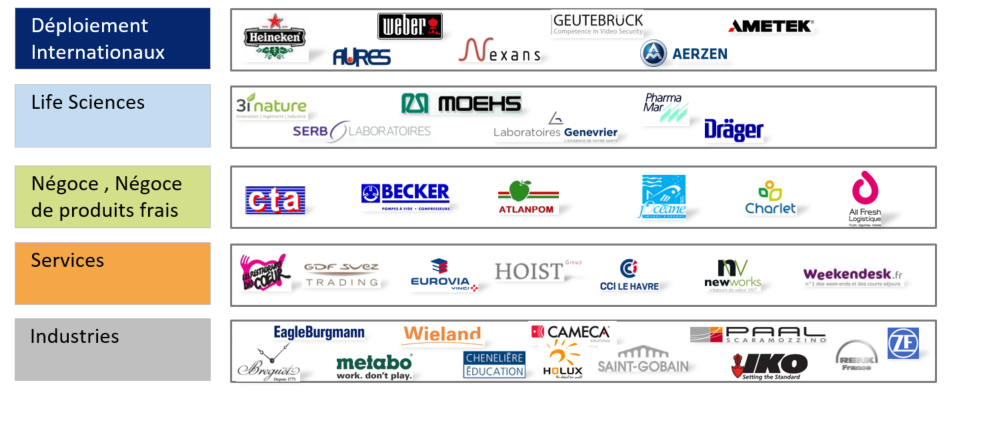
\includegraphics[scale=1]{images/figure2.png}
\underline{\textbf{Figure 2 : les différents clients par secteur}}
\end{center}

\section{Déroulement du stage}
	\subsection{Planning}
\hspace{1cm} J'ai commencé mon stage à Cosmo Consult France le 03 avril 2017.  Durant ma 1ère semaine ils m'ont fait visiter les locaux après les présentations avec les autres consultants. J’ai pris connaissance de la politique et de la structure de l’entreprise.\\

\hspace{1cm} Dès la semaine d’après, j’ai commencé à travailler sur mes missions. J’ai d’abord commencé à me documenter sur les principales activités de Cosmo qui s’active dans un secteur qui m’était inconnue. J’ai ainsi découvert le monde des ERP qui est un système d’information qui permet de gérer et suivre au quotidien, l’ensemble des informations et des services opérationnels d’une entreprise.\\

\hspace{1cm} La deuxième étape était de prendre connaissance des outils existants de Cosmo et de me familialiser avec et de m’imprégner dans l’entreprise. J’ai ainsi passé deux semaines de découvertes, de prises en main de nouveaux outils de travail et d’adaptation.\\

\hspace{1cm} J’ai eu l’occasion d’avoir une formation complète avec un consultant Cosmo Consult France sur Microsoft Dynamics NAV 2016.  J’ai aussi eu une formation animée du 20 au 21 juin par un consultant Cosmo Consult Allemagne sur les CCERP et qui a pour but d’expliquer les fonctionnements des CCERP.

	\subsection{Objectif du stage}
\hspace{1cm} L’objectif de mon stage était de travailler sur la mise en œuvre de solutions internes liées à la gestion de projets. J’avais deux grandes principales missions :
\begin{itemize}
	\item Une mission qui consiste à mettre en place une solution de planning consolidé.
	
	\item Une mission qui consiste à mettre en place une solution d’analyse des consommations de contrats type support.
\end{itemize}

\hspace{1cm} Je suis impliquée dans la phase d’étude du cahier des charges, d’étude de marché, de conception du projet d’intégration et si le temps me le permet du développement et du déploiement de la solution.\\

\hspace{1cm} A travers ces paragraphes, je vous parlerai principalement de la première mission qui avait une priorité plus élevée par rapport à la deuxième, quant à la deuxième mission, je devrais le commencer début juillet.

 % voir si on fait une new page ou bien 
 \newpage
\section{Missions}
	\subsection{Description de la mission}
\hspace{1cm} Pour la gestion de son planning et de la planification des projets, Cosmo Consult dispose de plusieurs outils qui travaillent séparément et indirectement dépendants.
Dans un premier temps chaque consultant remplit son planning dans un tableau Excel sur un site dédié à Cosmo Consult. Parallèlement ils remplissent ce même planning sur Outlook.\\

\hspace{1cm} Ce tableau contient le planning détaillé par jour des affectations projets sur les 3 mois à venir, voire \textit{annexe1}. Ensuite le contenu de tous les tableaux est recopié manuellement dans un tableau synthétique qui est un doublon du planning sur Outlook et qui présente le calendrier de tous les consultants avec les jours facturés par le client, les jours disponibles, les jours de vacances… Ce tableau sert aussi à estimer le chiffre d’affaire prévisionnel sur les trois prochains mois, voire \textit{annexe2}.
A la fin de ces saisies manuelles, une présentation de PowerPoint contenant le résumé de tous ces éléments est utilisée pour le BRM (Réunion de pilotage Groupe).\\

\hspace{1cm} Face à tous ces outils existants, qui se remplissent manuellement et répétitivement, Cosmo Consult souhaite améliorer sa gestion des plannings au sein de son siège et avoir une meilleure vision sur le déroulement de ses projets. \\

\hspace{1cm} Pour satisfaire à ses besoins il faut mettre en place un outil qui a pour objectif à terme de tout centraliser en un seul et unique outil afin de faciliter la saisie, de rendre plus simple la récupération des données et de permettre à chacun d’avoir une vue globale sur tous les plannings et de bien gérer la planification de projet.

	\subsection{Méthodes de travail}
\hspace{1cm} Cosmo Consult étant un groupe, prendre des décisions de relève pas seulement de Cosmo Consult France. Pour cela il y a plusieurs étapes à faire afin de convaincre les autres Cosmo et de faire accepter son outil de planning.\\

\hspace{1cm} Dans un premier temps, la vérification de l’existence d’un quelconque outil similaire dans les autres pays est nécessaire, voire obligatoire afin d’éviter des duplications.  J’ai organisé des réunions avec les allemands et les espagnols en présences de mes supérieurs.
\quad

\hspace{1cm} \underline{\textbf{\textit{Réunions avec les allemands}}}
\quad

\hspace{1cm} Une des méthodes de travail est de faire une réunion avec les allemands pour prendre connaissance de la façon de gérer leur planning, des outils qu’ils utilisent et voir si ça répond à nos besoins.\\

\hspace{1cm} Les allemands utilisent CCERP et autres outils pour gérer leur planification d'équipe et leur vérification de performance. La planification se fait dans Outlook par tout le monde. L’information de Outlook est transférée aux lignes de CCERP et à la feuille de planification Excel. Ensuite les chefs de projets vérifient ces informations dans Excel, et si nécessaire apportent des modifications manuelles dans Excel. La feuille de Excel est mise à jour pour les semaines précédentes de telle sorte qu’ils ont la planification de la semaine précédente et la planification pour la semaine prochaine. Ils utilisent également les résultats Excel pour leur « modèle de travail flexible », valable que pour les consultants en planification au projet.\\

\hspace{1cm} Pour organiser les réunions et les conseils d’administrations ils utilisent l’agenda sur OneNote Online. L’organisation des réunions hebdomadaires prend en compte la planification hebdomadaire du fichier Excel effectuée par les Team Leads par avance, les opérations du conseil d’administration et les ventes. Et les sujets suivants sont à l’ordre du jour : 
\begin{center}
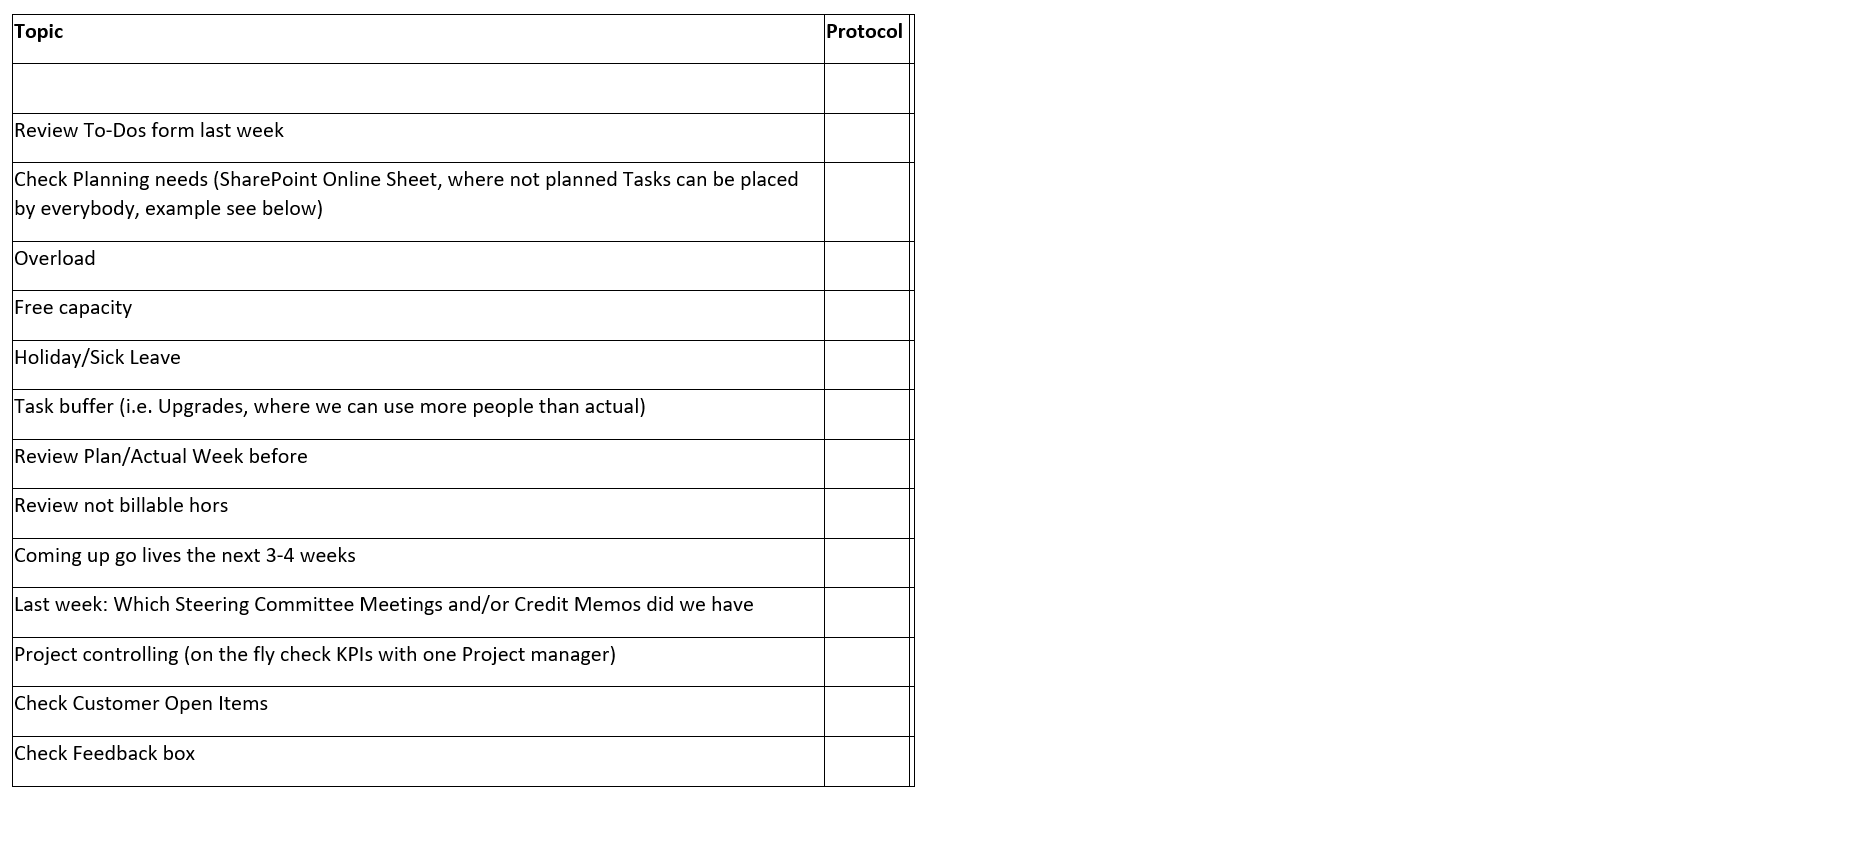
\includegraphics[scale=1]{images/tab1.png}
\end{center}

\hspace{1cm} Deux semaines après les réunions de planification, une petite réunion est organisée par les Team leads à l’avance et qui prend en compte la planification à long terme d’Excel (prévisions de 3 mois), les équipes et le conseil d’administration.  Les sujets suivants seront abordés :
\begin{center}
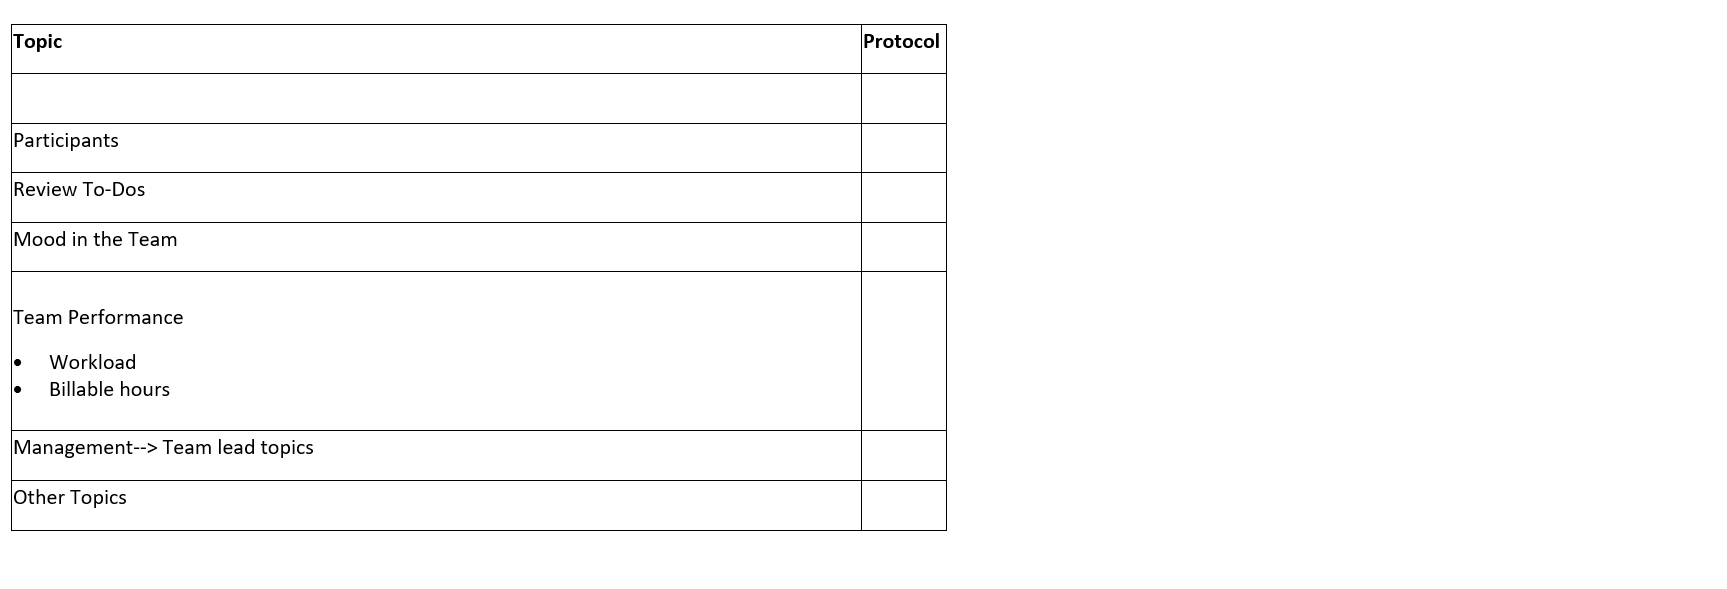
\includegraphics[scale=1]{images/tab2.png}
\end{center}

\hspace{1cm} Les allemands arrivent à gérer leur planning mais sont confrontés au même problème que nous à savoir l’utilisation de plusieurs outils, doublon avec les fichiers Excel, voir \textit{annexe3} et ils sont obligés de construire de petites équipes pour avoir un meilleur aperçu dessus, ce qui est une grande contrainte. Donc ils sont preneurs pour notre futur outil de planification.

\quad

\hspace{1cm} \underline{\textbf{\textit{Réunions avec les espagnols}}}
\quad

\hspace{1cm} Les espagnols utilisent à peu près les mêmes outils que les allemands. Chaque consultant remplit son planning du jour au jour. Ils font leurs exportations vers les fichiers Excel qu’ils vont gérer derrière et procèdent comme les allemands.  Cependant s’il y a des changements au cours d’un projet les chefs d’équipe sont obligés de tout modifier et de tout remettre en ordre. Ce qui est un vrai handicap pour la gestion de leur temps. 

	\subsection{Démarches de la résolution}
\hspace{1cm} \underline{\textbf{\textit{Collecte des besoins}}}
\quad

\hspace{1cm} Cosmo Consult France souhaite avoir les meilleures performances pour son outil de gestion des plannings. Un outil qui répondrait à tous leurs besoins. Je suis avant tout partie à la collecte des informations afin d’établir un tableau qui résume tous ce dont notre outil aura besoin. Pour ce faire j’ai utilisé la technique des \textbf{QQOQCPC} qui consiste à se poser les questions essentielles pour mener à bien un projet.\\

Ce tableau ci-dessous représente notre base de questions/réponses qui va nous aider à mettre en place notre outil de planning.

\begin{center}
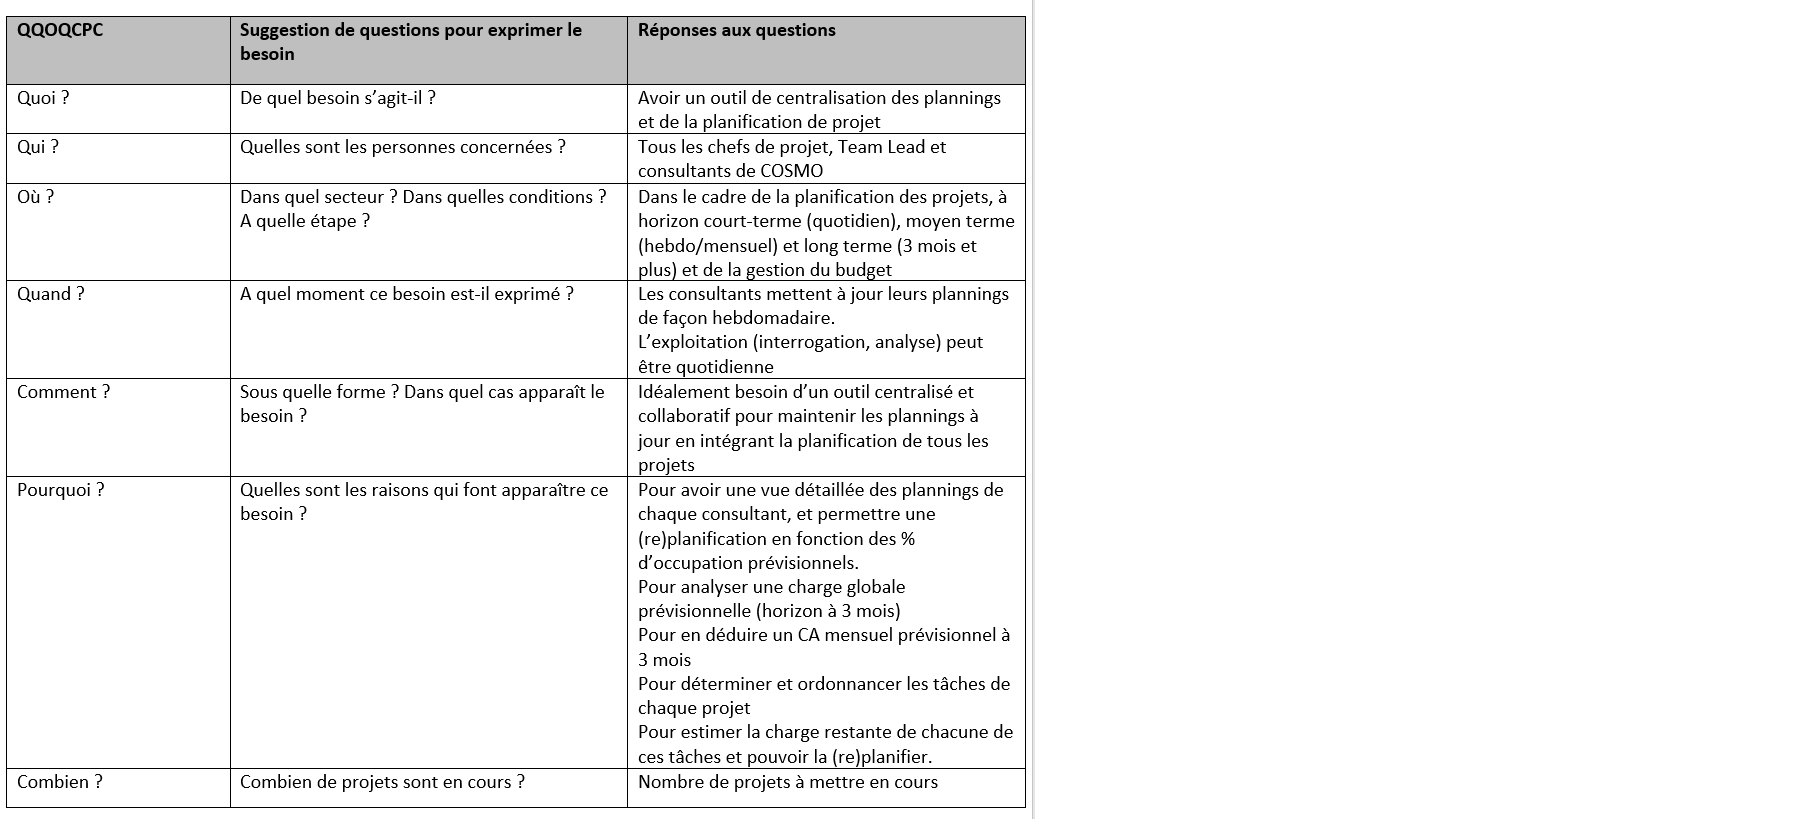
\includegraphics[scale=0.9]{images/tab3.png}
\end{center}

\hspace{1cm} \underline{\textbf{\textit{Définition du périmètre}}}
\quad

\hspace{1cm} A partir de la synthèse de ces besoins et avec l’aide de mon tuteur j’ai pu établir les fonctions de services liées au produit. Ces fonctionnalités sont fondamentales pour le choix de l’outil. Les principales fonctions indispensables pour notre outil de plannings sont :  

\begin{center}
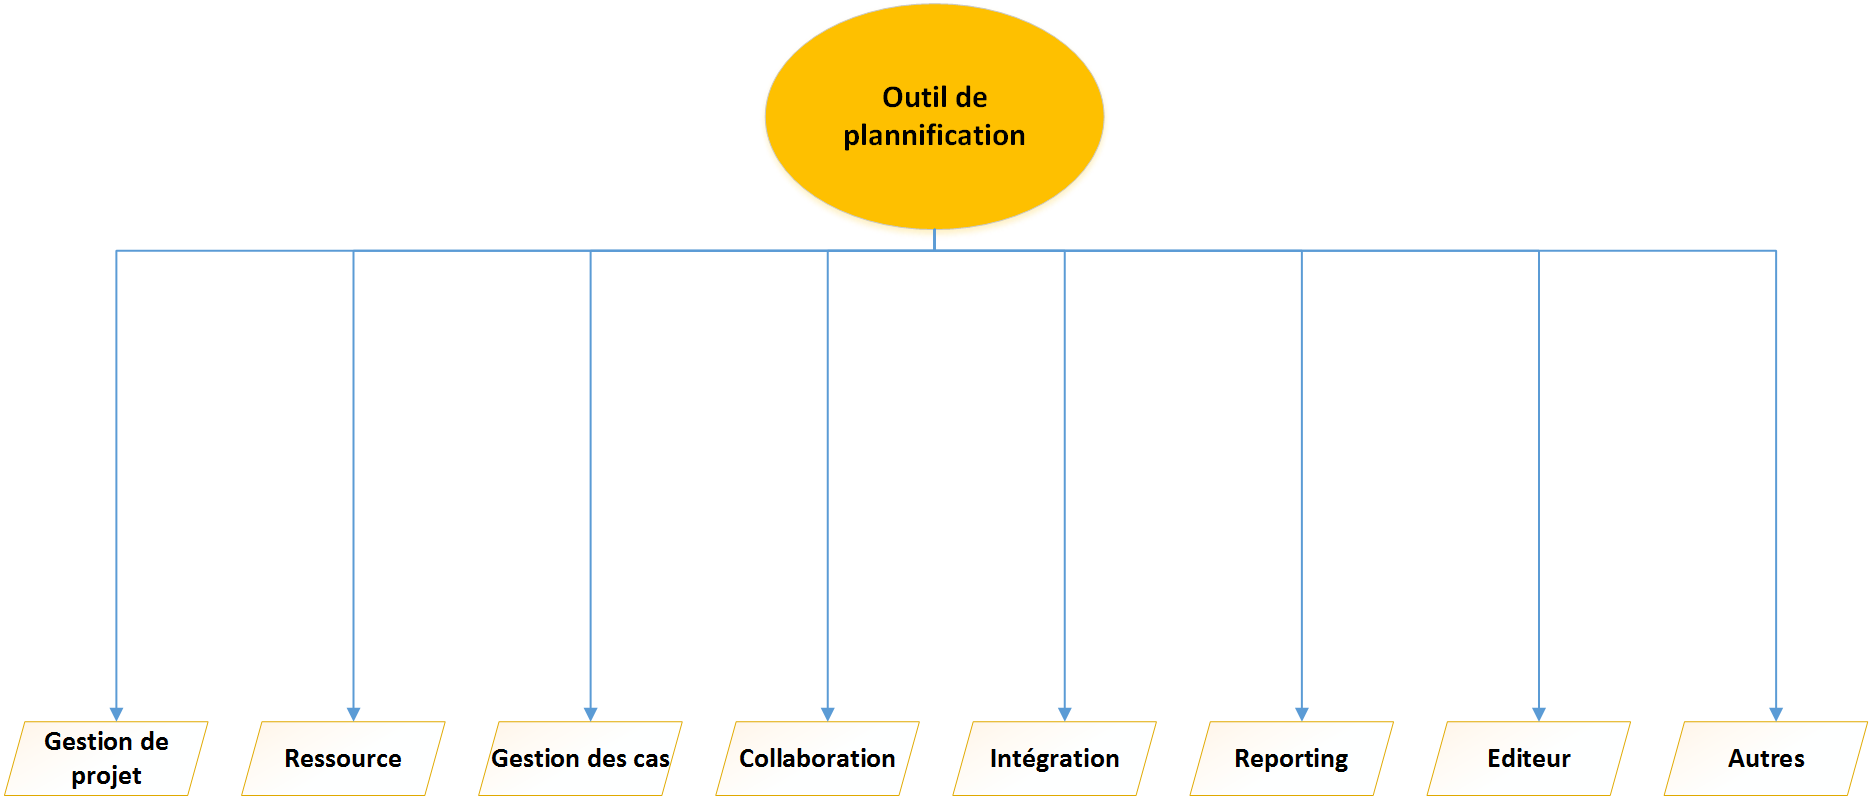
\includegraphics[scale=0.5]{images/figure3.png} \

\underline{\textbf{Figure 3 : Les principales fonctionnalités}}
\end{center}
\quad

Ces différentes fonctionnalités sont subdivisées en sous-parties qui assurent le bon fonctionnement de notre outil. Nous allons les voir plus en détail, et mieux développer leurs utilités.\\

\begin{center}
\underline{\textbf{Gestion de projet}} 
\end{center}
Cette fonctionnalité est la plus importante de toutes. En effet nous y retrouvons : 
\begin{itemize}
	\item \textbf{La planification automatique} nous permet de calculer la planification basée sur l’effort qui est l’unité de travail mis pour accomplir une tâche ciblée et la planification basée sur la durée qui est le temps mis pour accomplir l’activité attribuée en fonction des ressources allouées au projet.
	
	\item \textbf{La gestion des unités} qui nous donne le nombre de temps mis en unité d’heure, de jour ou bien de pourcentage.
	
	\item \textbf{Le WBS} qui nous aide à organiser le projet, en définissant la totalité du contenu, et servant de référence pour planifier les activités et établir le budget prévisionnel. Il aide également à guider la gestion des risques, ou identifier les acquisitions nécessaires et nous permet également de déléguer la mission confiée à chaque consultant. 
	
	\item\textbf{ La saisie des temps} qui consiste à donner la possibilité de rentrer le temps de travail réalisé et le temps de travail qui reste à faire. Ces saisies permettront de bien suivre le projet et de gérer les délais de livraison. 
	
	\item \textbf{L’analyse des projets} donne une visibilité globale du projet. Cette fonctionnalité s’ouvre sur quatre grandes « sous-fonctionnalités » :
	
	\begin{itemize}
		\item \textbf{Plan de charge} des ressources nous fait une synthèse des temps passés et planifiés sur les projets. 
		
		\item \textbf{Affichage Gantt} : à partir du diagramme de Gantt qui nous permet de représenter visuellement l’état d’avancement des tâches de chaque projet. Ce diagramme est très important pour notre outil car il nous donne la possibilité de savoir en un coup d’œil :
		
		\begin{itemize}
			\item \textit{Les différentes tâches à envisager}
			\item \textit{La date de début et la date de fin de chaque tâche}
			\item \textit{La durée escomptée de chaque tâche}
			\item \textit{Le chevauchement des tâches et la durée du chevauchement}
			\item \textit{La date de début et la date de fin du projet dans son ensemble}
		\end{itemize}
		
		\item \textbf{Analyse de plusieurs projets} : il faut un outil qui nous donne une vue d’ensemble et détaillée sur les autres projets.
	\end{itemize}
	
	\item Le référentiel projet : il regroupe les informations de base, le rattachement d’un projet à un client, le regroupement des projets et le lien entre ces projets.
	
	\item D’autres fonctionnalités :  nous pouvons aussi avoir l’archivage des projets dans notre outil pour des consultations et obtenir des informations.
\end{itemize}

\newpage
\begin{center}
\underline{\textbf{La structure de la fonctionnalité \textit{Gestion de projet} ci-dessous :}}
\end{center}

\begin{center}
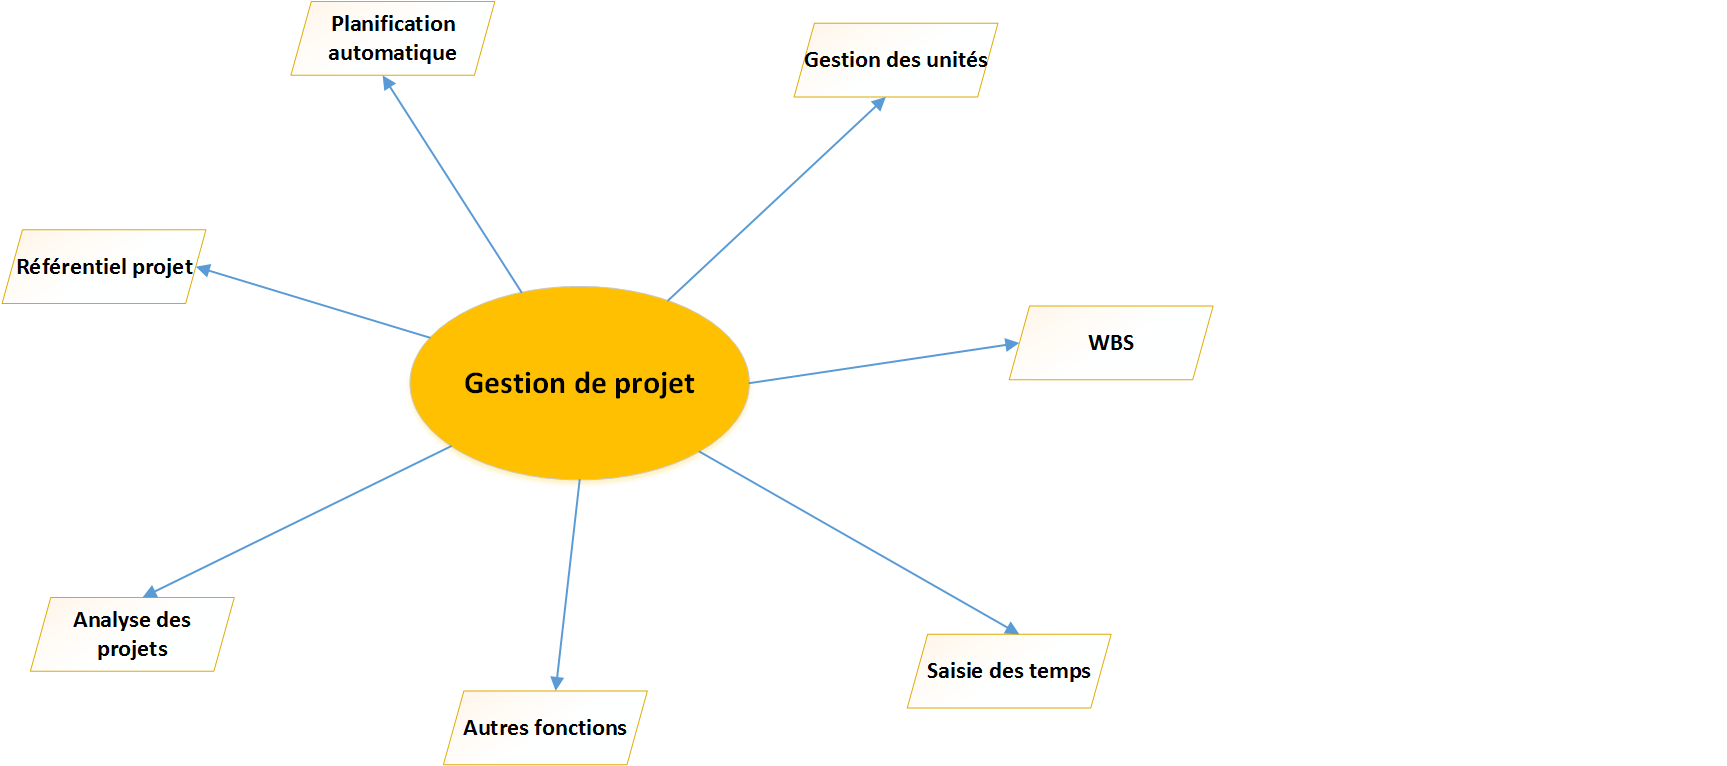
\includegraphics[scale=0.8]{images/figure4.png} 
\quad

\underline{\textbf{Figure 4 : Gestion de projet}}
\end{center}
\quad

\begin{center}
\underline{ \textbf{Ressource} }
\end{center}
\hspace{1cm} Pour une bonne gestion d’un projet il faut avoir la possibilité de vérifier ses ressources et de les affecter sur les tâches appropriées. Ces caractéristiques suivantes nous décrivent nos attentes par rapport à l’outil :
\begin{itemize}
	\item \textbf{Le référentiel des ressources} qui regroupe toutes les informations de base à savoir l’email, l’identifiant, le nom …
	
	\item \textbf{La gestion des compétences} : Pour ne pas affecter des tâches à des ressources qui ne seront pas à la hauteur ou bien qui auront des difficultés à bien faire le travail, il est essentiel de vérifier les compétences de ses ressources afin de savoir quelle tâche affectée à quelle ressource. 

	\item \textbf{La gestion des capacités et des disponibilités} : avant d’affecter une ressource à une tâche il faut aussi voir ses disponibilités, voir si elle peut ou pas travailler sur le projet pour ne pas avoir des retards de livraisons ou des arrêts de projet. 

	\item \textbf{L’affection des ressources} :  un projet a besoin de ressources dessus pour être mené jusqu’au bout. Donc cette fonctionnalité nous permet juste d’avoir des personnes pour faire le projet.

	\item \textbf{La gestion des groupes et des équipes de ressources} : après avoir affecté nos ressources sur les tâches, il faut aussi savoir gérer les groupes, les imprévus et les demandes.
\end{itemize}

\begin{center}
\underline{\textbf{La structure de la fonctionnalité \textit{Ressource} ci-dessous :}}
\end{center}
\begin{center}
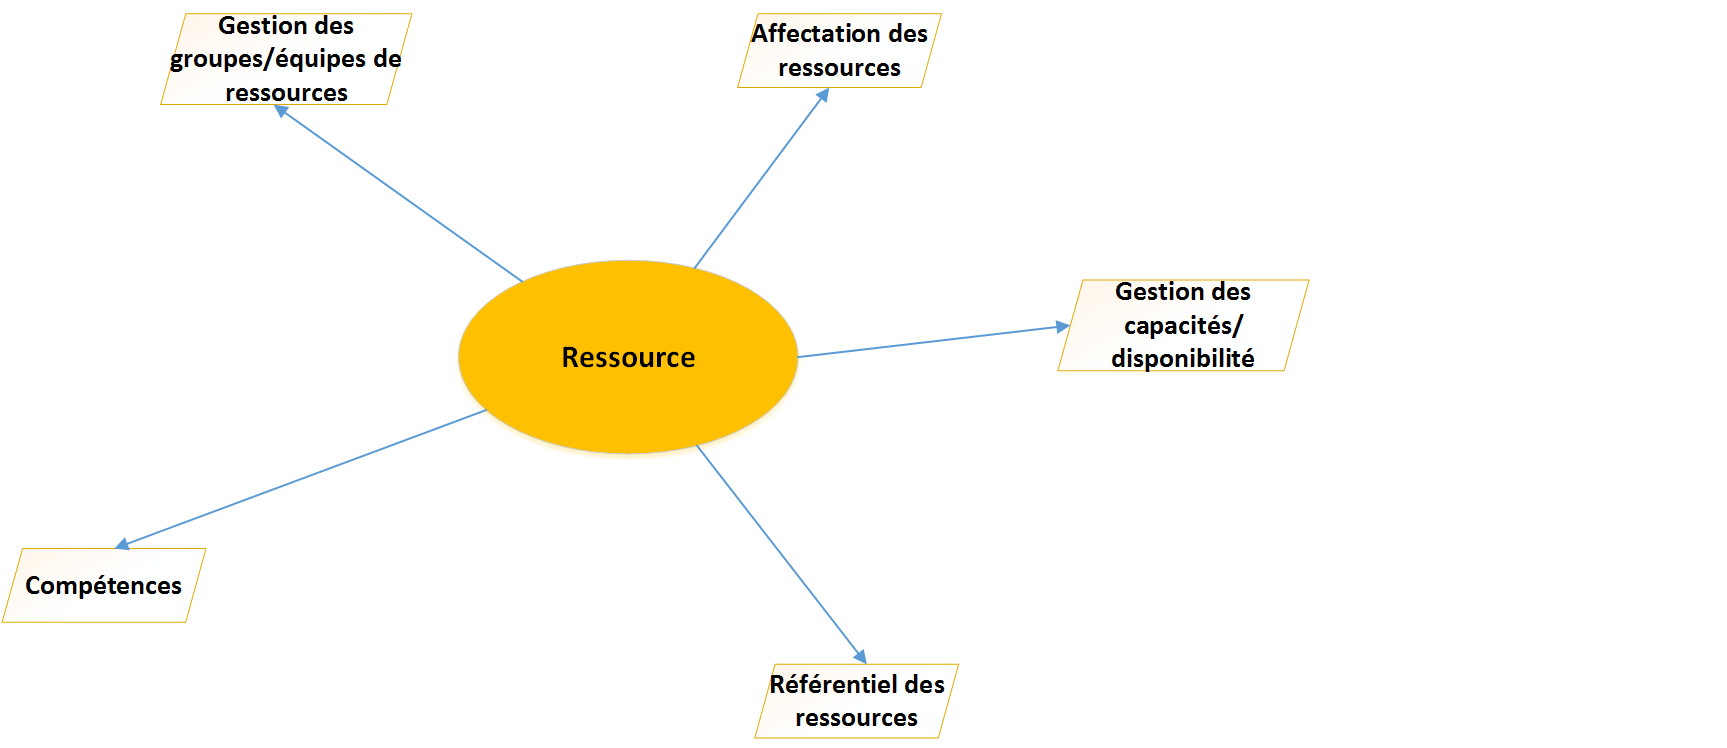
\includegraphics[scale=0.7]{images/figure5.png} 
\quad

\underline{\textbf{Figure 5 : Ressource}}
\end{center}

\newpage
\begin{center}
\underline{\textbf{Gestion des cas}} 
\end{center}

\hspace{1cm} Dans un projet il faut savoir gérer les risques qui peuvent être néfaste pour le projet. Les incidents aussi doivent être détectés et résolus à temps. Voyons un peu plus en détail la gestion des cas : 
\begin{itemize}
	\item \textbf{La gestion des demandes} : qui gère toutes les demandes concernant un projet durant tout son cycle.

	\item \textbf{La gestion des incidents} : pareil que les demandes, mais plus de suivis
	
	\item \textbf{La gestion des risques} : qui nous permet de suivre et de bien gérer les risques qui adviennent souvent dans les projets.

	\item \textbf{Le flux de travail} : dans cette partie, nous gérons les statuts des demandes, les suivis de ses statuts jusqu’à leur validation. Nous avons aussi besoin de transformer certains cas en tâche.

	\item \textbf{L’assignation des cas} : qui nous permet d’assigner des cas à des tâches afin de les traiter et d’assigner ces cas à des ressources pour qu’ils puissent les résoudre.
\end{itemize}

\begin{center}
\underline{\textbf{La structure de la fonctionnalité \textit{Gestion des cas} ci-dessous :}}
\end{center}
\begin{center}
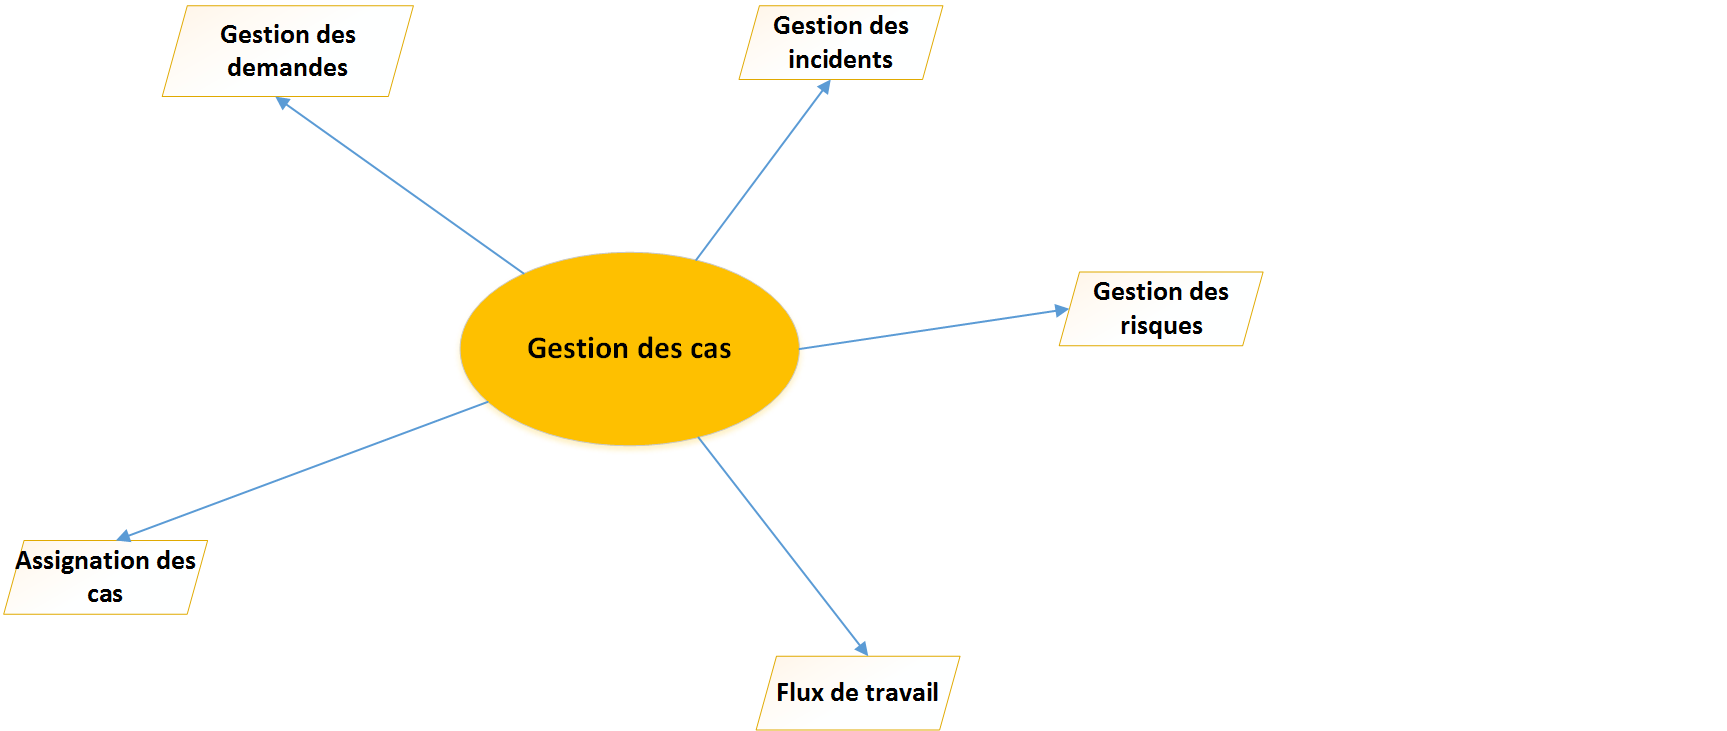
\includegraphics[scale=0.7]{images/figure6.png} 
\quad

\underline{\textbf{Figure 6 : Gestion des cas}}
\end{center}
\quad

\begin{center}
\underline{\textbf{Collaboration}} 
\end{center}

\hspace{1cm} La collaboration est le lien sacré entre nous et les clients qui ont eu la confiance de nous confier leurs projets. Il est primordial de les tenir au courant de l’avancement de leurs projets, et si souhaité de leur faire des synthèses sur ce qui se passe. 

\begin{itemize}
	\item \textbf{L’intégration e-mail entrants} : pour communiquer avec les clients par mails. Ils peuvent aussi créer des cas à partir des mails qui seront pris en charge.
	
	\item \textbf{Le partage d’informations} : qui peut se faire par mail ou par lien.
	
	\item \textbf{Le portail client} : qui permet aux clients d’accéder aux projets, aux incidents et de pouvoir les soumettre pour qu’ils soient traités.
\end{itemize}

\begin{center}
\underline{\textbf{La structure de la fonctionnalité \textit{Collaboration} ci-dessous :}}
\end{center}
\quad

\begin{center}
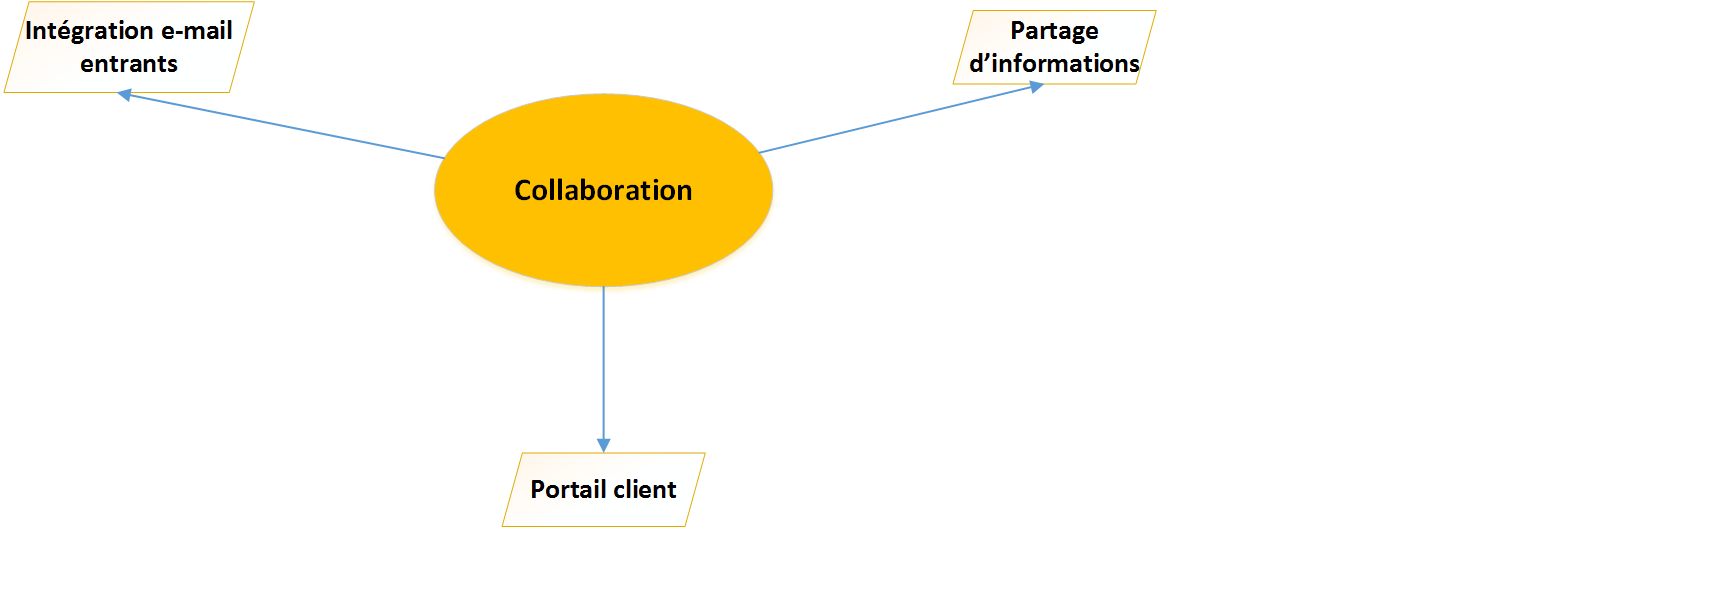
\includegraphics[scale=0.8]{images/figure7.png} 
\quad

\underline{\textbf{Figure 7 : Collaboration}}
\end{center}

\newpage
\begin{center}
\underline{\textbf{Intégration}} 
\end{center}

\hspace{1cm} Notre outil a besoin d’intégrations de certaines fonctionnalités pour mieux fonctionner et nous permettre de travailler dans un bon confort. Les principales intégrations nécessaires pour notre outil sont.

\begin{itemize}
	\item \textbf{API }: qui nous permettra de pouvoir accéder aux projets, aux ressources et aux feuilles de temps.

	\item \textbf{SSO support} : qui implique l’intégration de Active Directory qui nous garantit un système de service centralisé d’identification et de l’intégration de Office 365. 

	\item \textbf{MS Project} : qui est un grand classique dans la gestion de projet. Il nous permet de piloter et de planifier les projets ainsi que de communiquer les données des projets.

	\item \textbf{L’intégration Outlook} : qui synchronise les tâches des projets directement avec Outlook, de même que le planning des consultants. 

	\item \textbf{MS Excel} : l’exportation et l’importation des données nous aident à extraire le contenu, la synthèse de nos projets ou d’envoyer des résumés à partir d’Excel. 

	\item \textbf{Gestion des documents} : avoir le monopole sur tous les documents d’un projet est préférable en intégrant le SharePoint et le OneDrive afin de partager les documents des projets entre consultants en toute sécurité. 

	\item \textbf{Application sur mobile} : l’idéal serait en effet de pouvoir emporte tous ses projets ou que vous soyez. Et mieux même, d’avoir la possibilité de les déployer sur Android et /ou sur IOS.

	\item \textbf{L’ajout des champs spécifiques} : cette intégration nous permet facilement d’ajouter des projets et des ressources.
\end{itemize}

\newpage
\begin{center}
\underline{\textbf{La structure de la fonctionnalité \textit{Intégration} ci-dessous :}}
\end{center}
\begin{center}
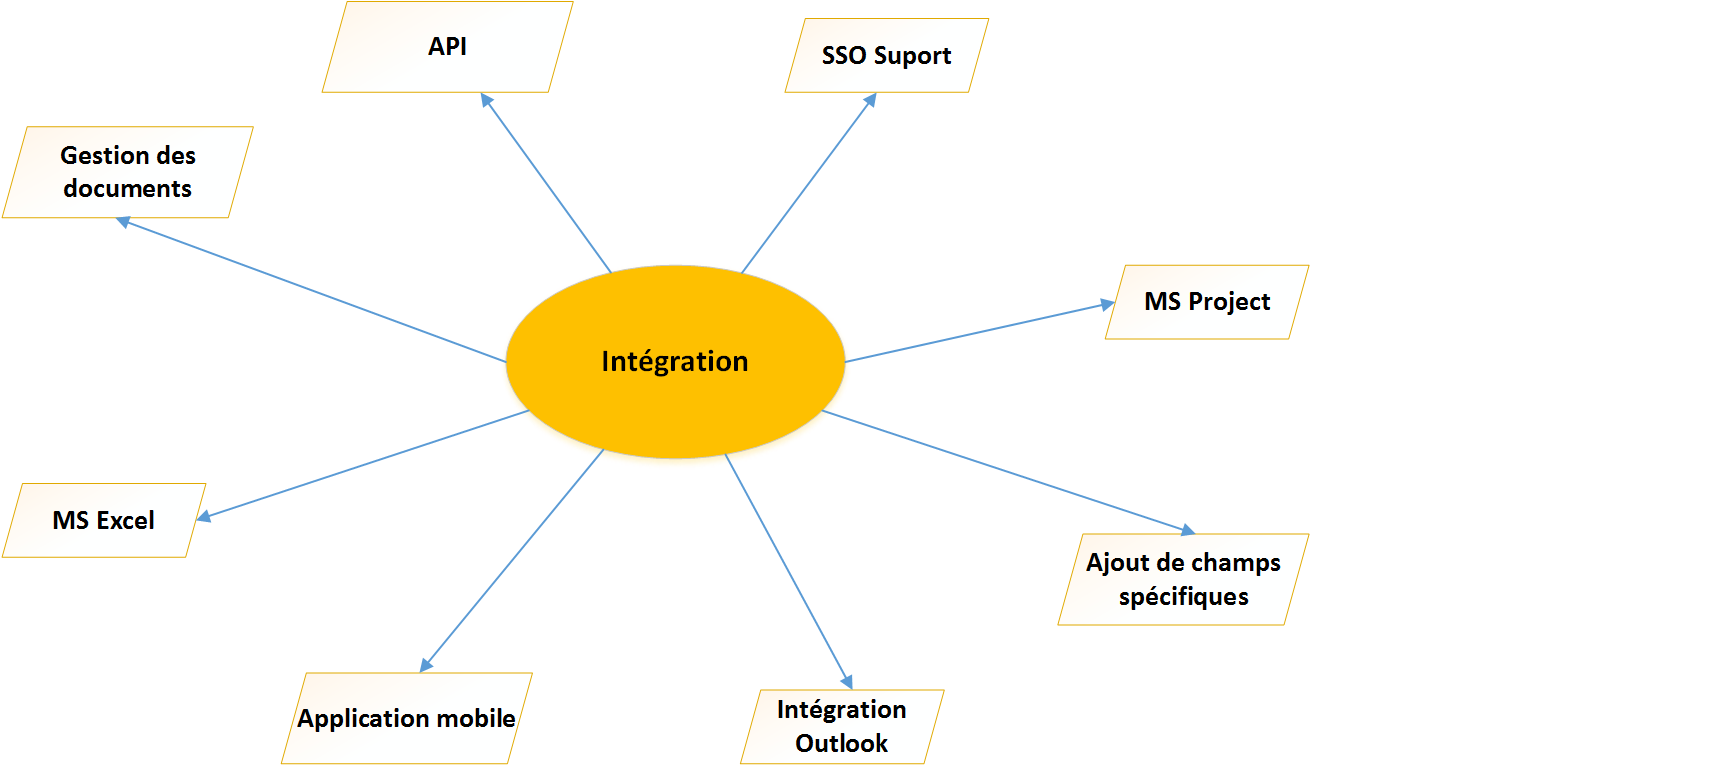
\includegraphics[scale=0.7]{images/figure8.png} 
\quad

\underline{\textbf{Figure 8 : Intégration}}
\end{center}
\quad
---
\begin{center}
\underline{\textbf{Reporting}} 
\end{center}

\hspace{1cm} Le reporting nous permet de faire des suivis sur les pôles essentiels de nos projets. Ainsi nous avons les fonctionnalités suivantes : 

\begin{itemize}
	\item \textbf{Le suivi des projets et des ressources} : un reporting sur les projets et les ressources nous aide à connaitre l’état de nos projets.

	\item \textbf{Le suivi des risques }: pour garder un œil sur les risques, afin de mieux les gérer.

	\item \textbf{Le suivi des coûts} : bien suivre les coûts dans un projet est indispensable. Cette fonctionnalité nous permet ainsi de connaître l’état de notre budget et de contrôler les coûts.

	\item \textbf{Le suivi des cas} : pour être tenu au courant de tous les cas.
\end{itemize}

\begin{center}
\underline{\textbf{La structure de la fonctionnalité \textit{Reporting}  ci-dessous :}}
\end{center}
\begin{center}
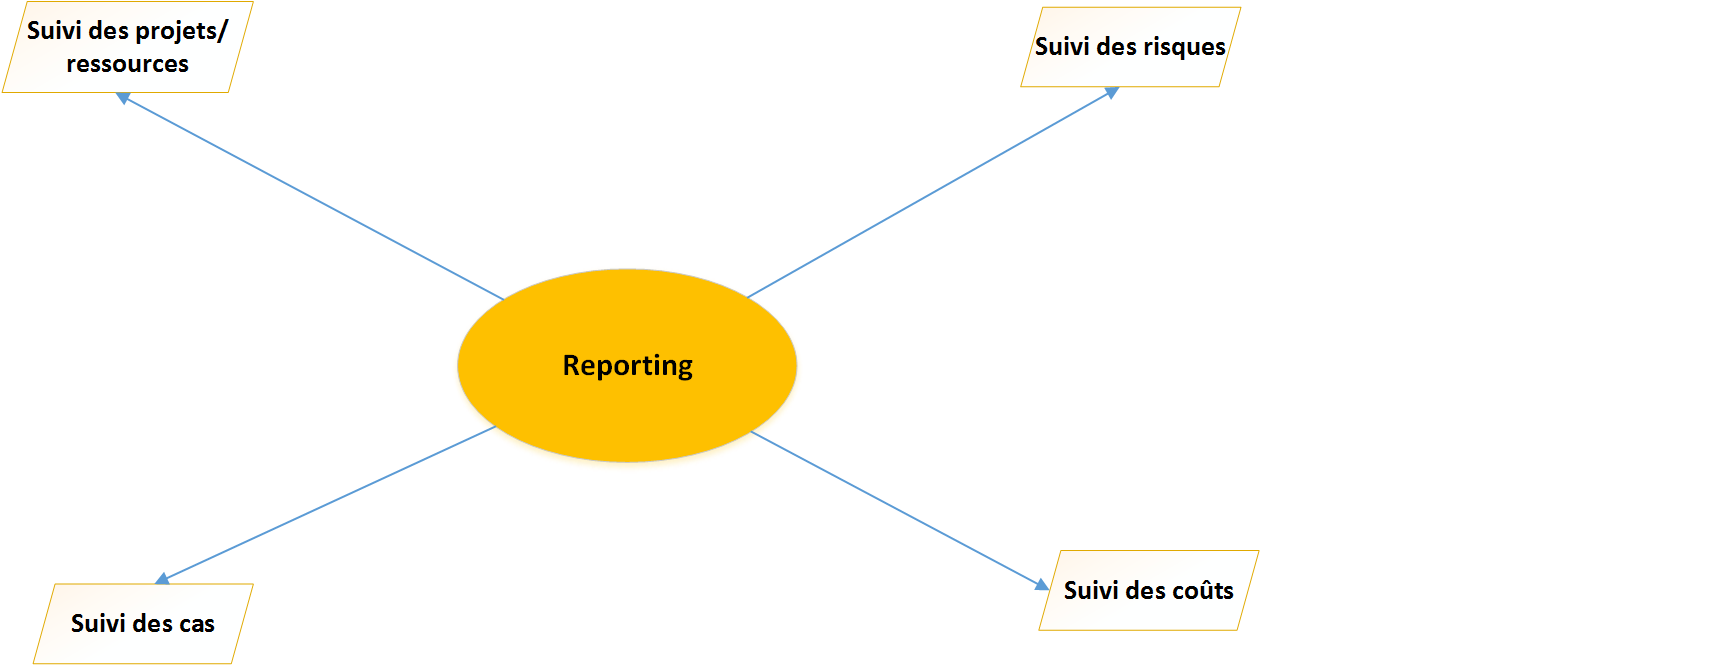
\includegraphics[scale=0.8]{images/figure9.png} 
\quad

\underline{\textbf{Figure 9 : Reporting}}
\end{center}
\quad

\begin{center}
\underline{\textbf{Editeur}} 
\end{center}

\hspace{1cm} Il faut tenir compte du statut de l’éditeur pour la pérennité de l’outil à savoir :

\begin{itemize}
	\item \textbf{La Raison sociale} : il faut connaître le lieu où se trouve la société de l’éditeur

	\item \textbf{La filiale} : pour s’assurer de la taille de la société

	\item\textbf{ La date de création de la société} : qui nous permet vérifier l’ancienneté de la société.

	\item \textbf{L’effectif total de la société} : le nombre d’effectif de la société nous garantit aussi de la taille et du sérieux de notre éditeur.

	\item Les modalités de support : avoir un support pour régler les éventuels problèmes techniques qui peuvent survenir sur l’outil
\end{itemize}

\newpage
\begin{center}
\underline{\textbf{La structure de la fonctionnalité \textit{Editeur} ci-dessous :}}
\end{center}

\begin{center}
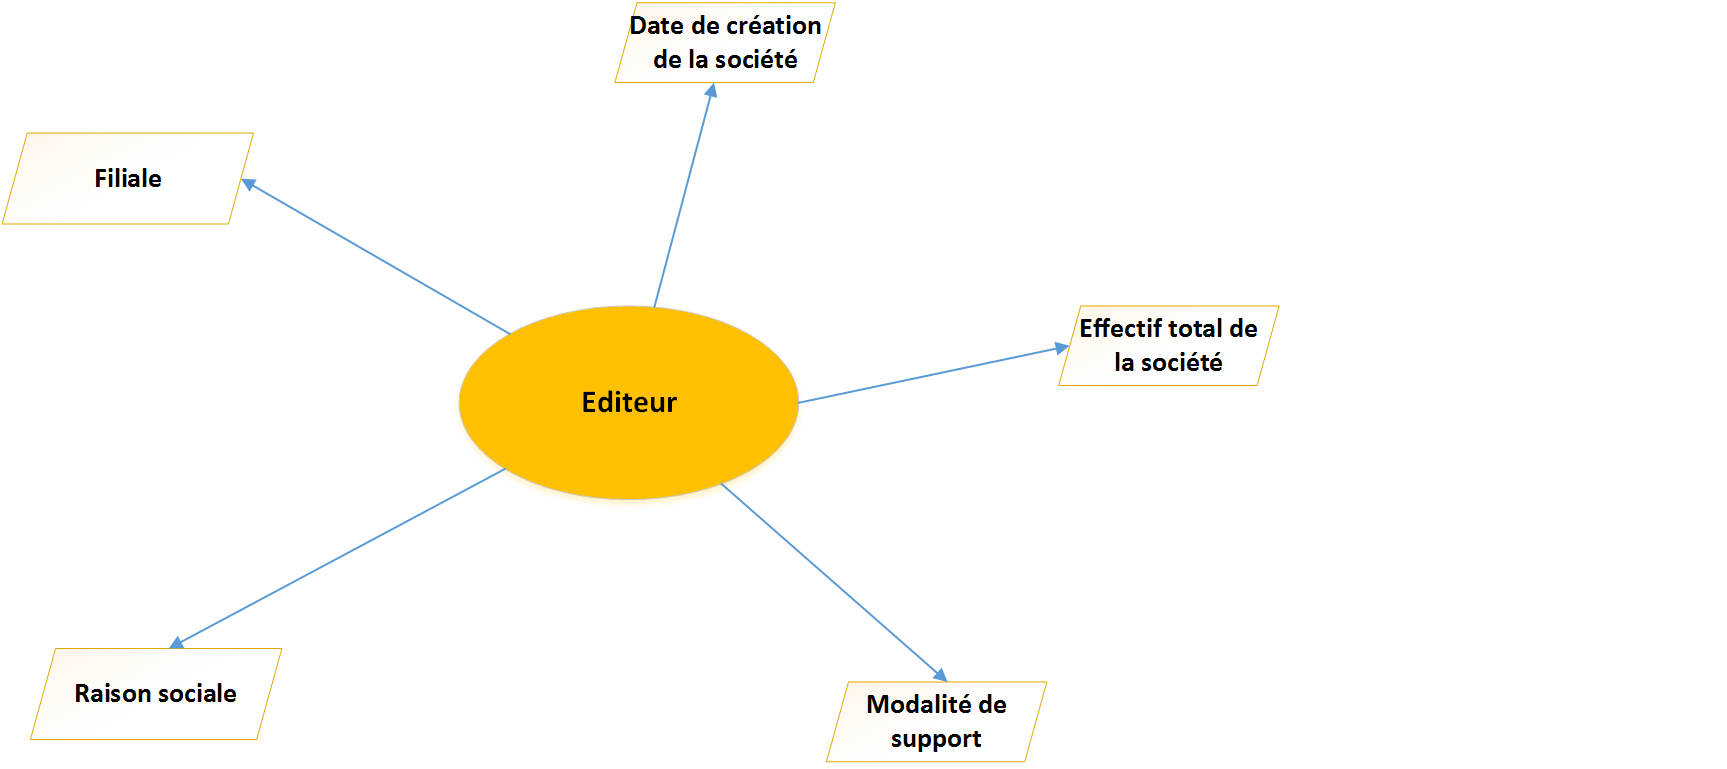
\includegraphics[scale=0.7]{images/figure10.png} 
\quad

\underline{\textbf{Figure 10 : Editeur}}
\end{center}
\quad

\begin{center}
\underline{\textbf{Autres fonctionnalités}} 
\end{center}

\hspace{1cm} Ces fonctionnalités de plus sont aussi importantes que celles citées un peu plus en haut. Nous aurons besoin :

\begin{itemize}
	\item \textbf{Le mode de déploiement} : nous avons deux types de mode :
	\begin{itemize}
		\item \textbf{Cloud} : permet aux consultants d’accéder à l’outil par le réseau et lui permet aussi de gérer et contrôler les paramètres de l’application
		
		\item \textbf{On Premise} : qui nécessite l’installation sur les serveurs de l’entreprise et donc d’acquérir définitivement l’achat des licences.
	\end{itemize}
	
	\item \textbf{La gestion de permission et de sécurité} : sécuriser notre outil fait partie des précautions à prendre par mesure.

	\item \textbf{Le type de client} : s’assurer si nous avons affaire à un client Web ou Application Windows

	\item \textbf{La langue supportée} : tenir compte de la langue supportée par l’outil s’assurer si c’est utilisable par Cosmo Consult et son groupe. 

	\item \textbf{Le tarif} : afin de pouvoir faire valider notre choix par le groupe Cosmo, il nous faut aussi les prix et modalité d’abonnement de l’outil.	
\end{itemize}
\quad

\begin{center}
\underline{\textbf{La structure de la fonctionnalité \textit{Autres} ci-dessous :}}
\end{center}
\begin{center}
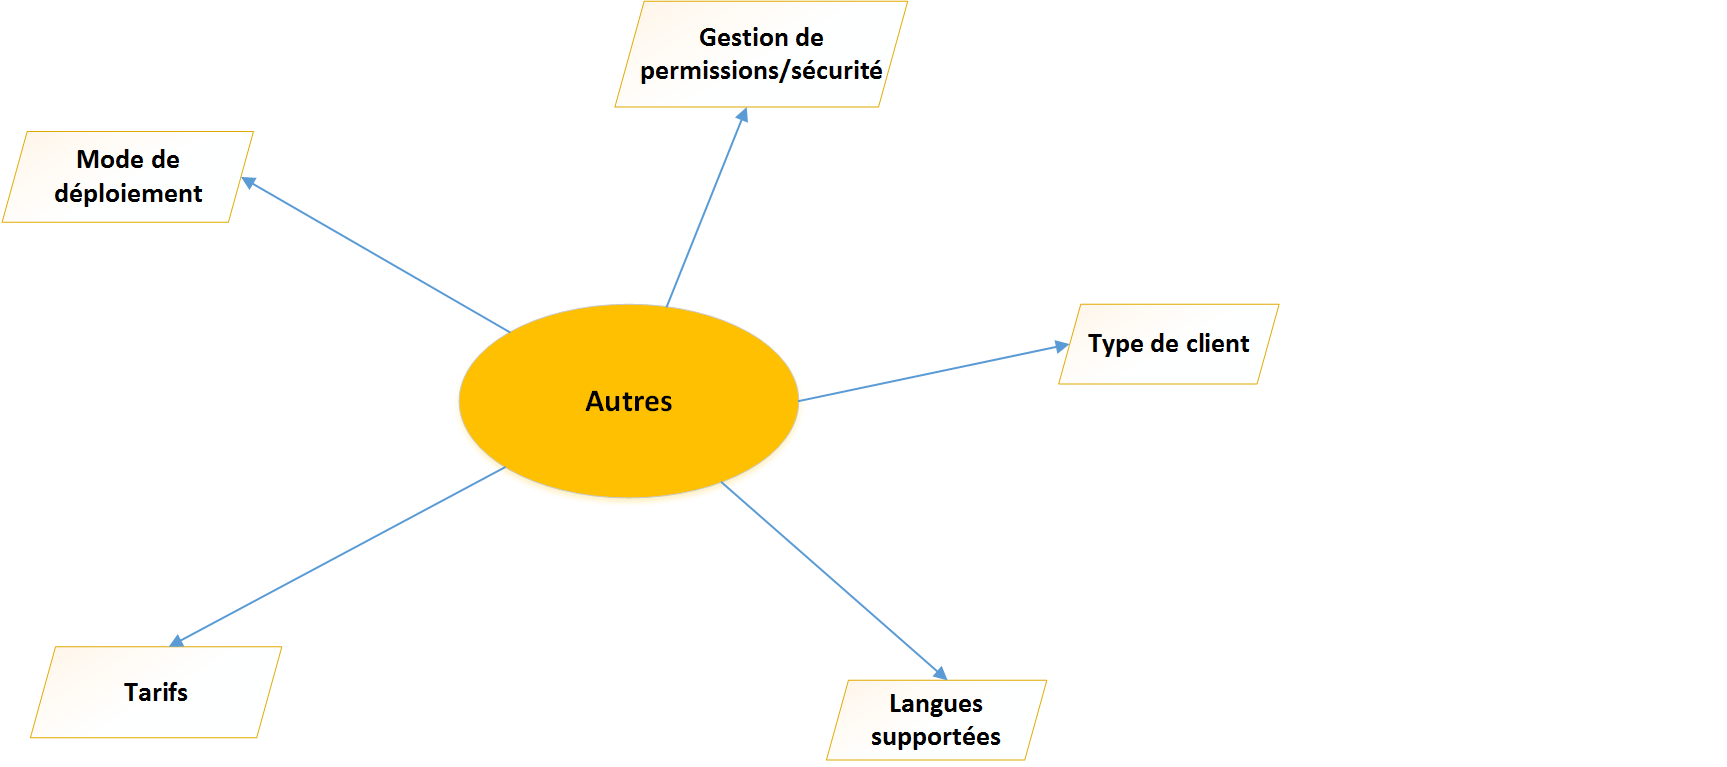
\includegraphics[scale=0.7]{images/figure11.png} 
\quad

\underline{\textbf{Figure 11 : Autres fonctionnalités}}
\end{center}
\quad

\hspace{1cm} L’outil souhaité a ses complexités et ces fonctionnalités détaillées ci-dessus permettent de contourner les difficultés et conduisent à la satisfaction de notre produit.
\quad

\hspace{1cm} \underline{\textbf{\textit{Etude de marché}}}
\quad

\hspace{1cm}Pour trouver le meilleur outil sur le marché adapté à nos besoins, j’ai établi un tableau comparatif composé de :
\begin{itemize}
	\item Une colonne \textbf{Besoins} qui énumère toutes nos fonctionnalités souhaitées, préalablement expliquées au-dessus.

	\item Une ligne \textbf{Solutions} qui récupère les outils que nous avons choisi qui, même s’ils ne remplissent pas tous les critères, se rapprochent le plus possible de notre souhait. 
\end{itemize}

Le récapitulatif des fonctionnalités que proposent les outils sur le marché en fonction de nos attentes:
\begin{center}
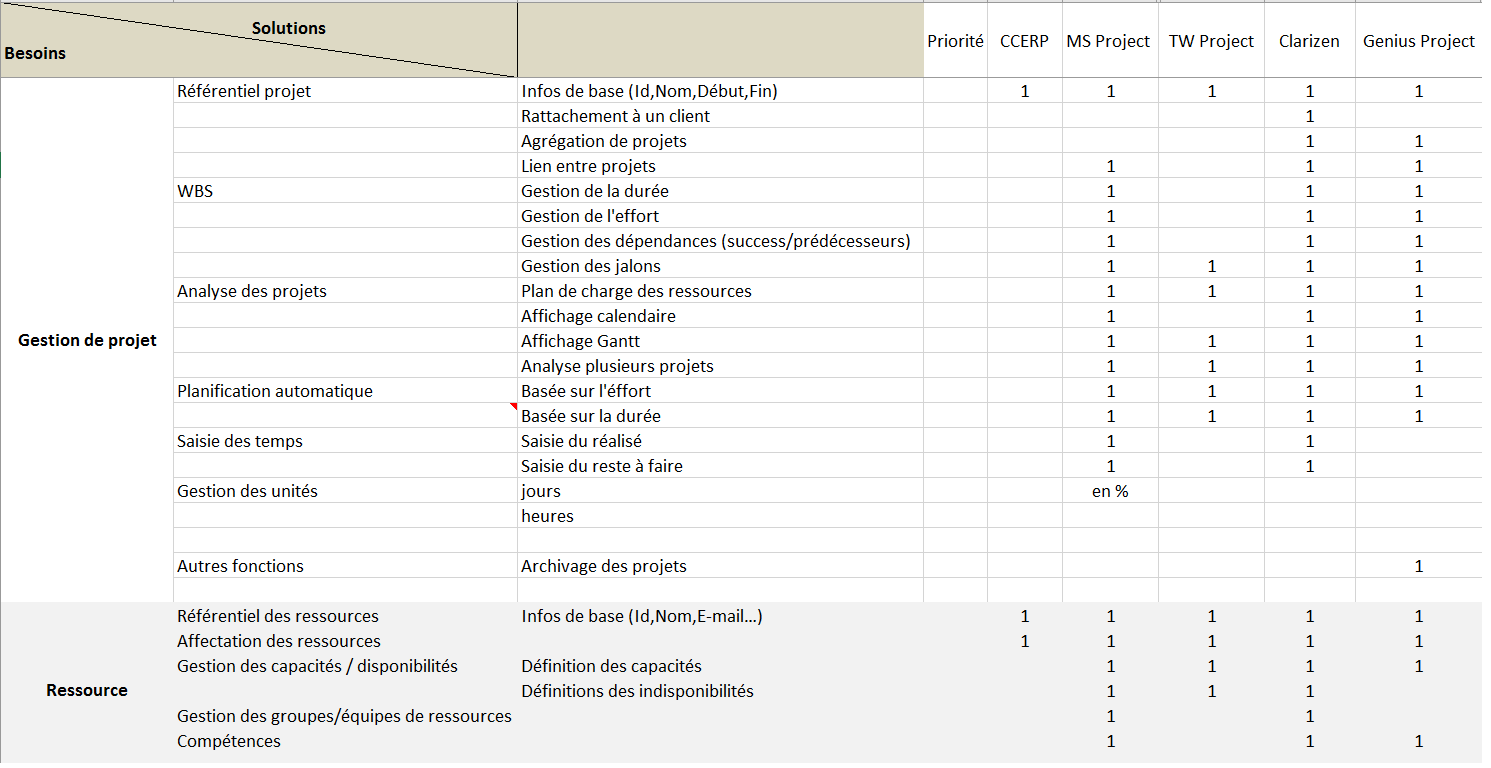
\includegraphics[scale=0.6]{images/figure12.png}
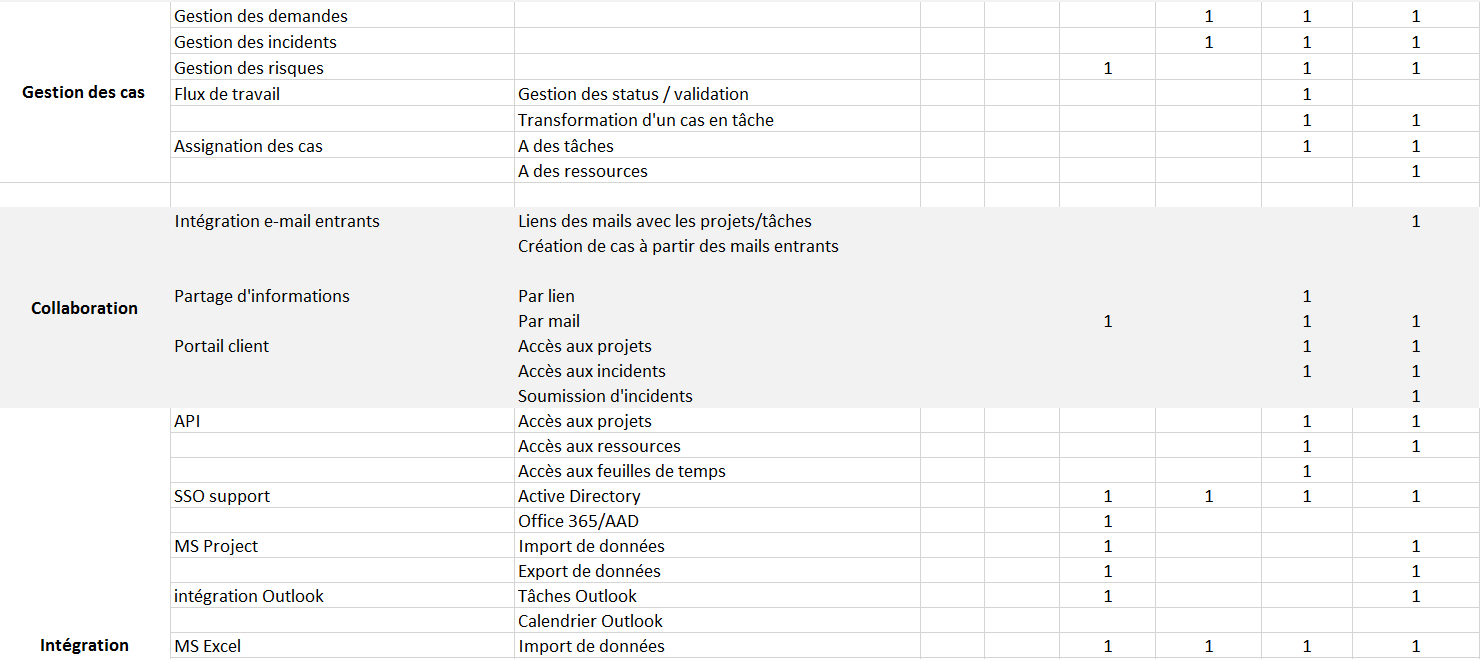
\includegraphics[scale=0.6]{images/figure13.png}
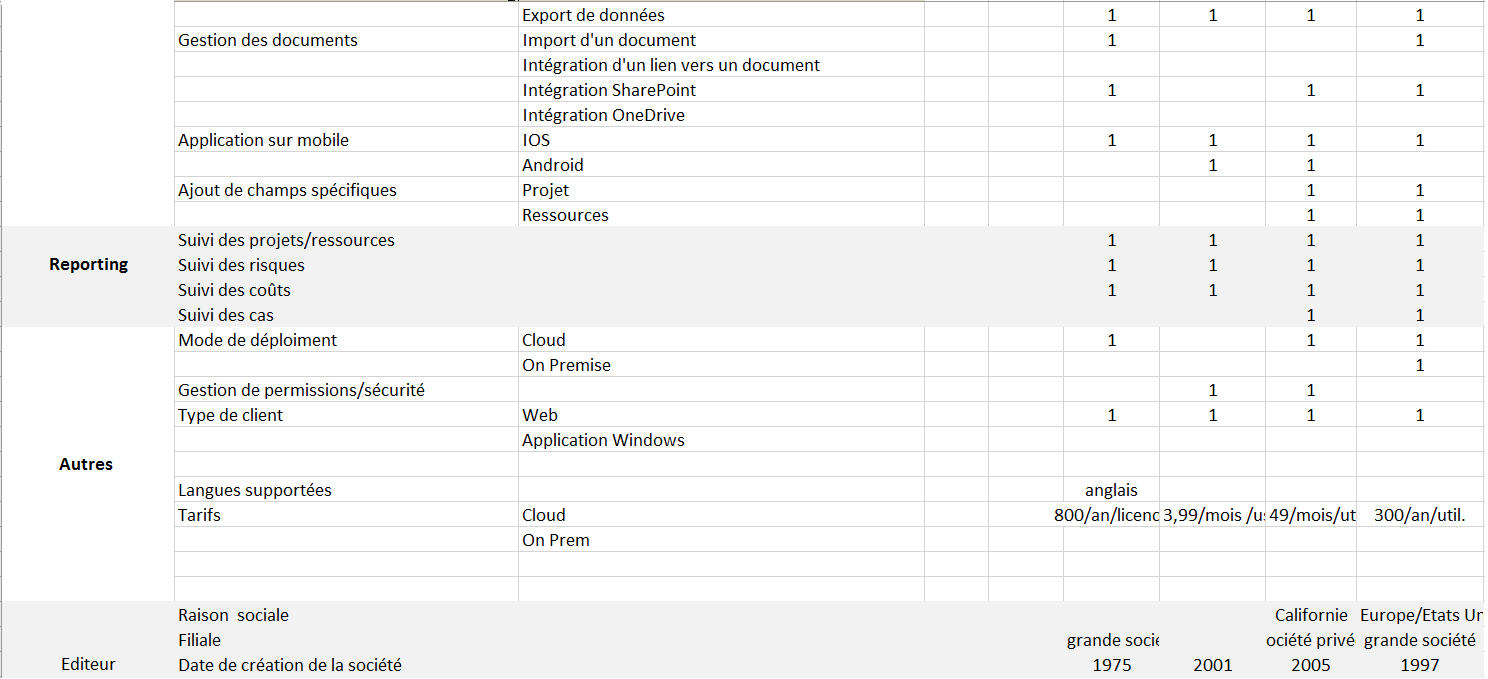
\includegraphics[scale=0.6]{images/figure14.png}
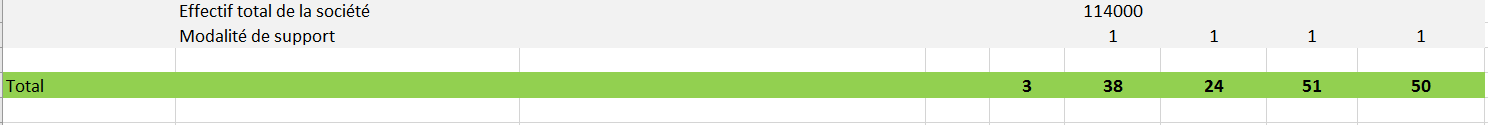
\includegraphics[scale=0.6]{images/figure15.png}    
\quad

\underline{\textbf{Figure 11 : Autres fonctionnalités}}
\end{center}

\hspace{1cm} \underline{\textbf{\textit{Choix final}}}
\quad

\hspace{1cm} Après l’étude de nos besoins et les outils que dispose le marché, il n’est pas facile de prendre une décision. Chaque outil offre des services différents et n’ont pas tous les mêmes priorités et l’impact sur notre produit souhaité.\\

\hspace{1cm} Cependant si nous nous basons sur l’efficacité d’un outil de gestion de projet et sur la large gamme de fonctionnalités proposées, notre choix se penche sur \textbf{\textit{Clarizen}}.\\
En effet \textbf{\textit{Clarizen, Inc}}. est une grande société de logiciel de gestion de projet très connue qui nous propose des prix très abordables et remplit plusieurs de nos critères. C’est aussi un logiciel qui est assez facile à manipuler avec une jolie interface.\\

\hspace{1cm} Cependant le choix définitif n’est pas encore fait. Nous devrons expliquer au reste du groupe notre penchant sur Clarizen et les motivations qui nous ont poussé à en décider ainsi. Et d’ici là je continue mes recherches afin de détecter le meilleur outil possible.

\newpage		
\section{Bilan}
\hspace{1cm} La mise en place de l’outil de gestion de projet touche presque à sa fin. J’ai eu trois mois à étudier le terrain, à faire des recherches, à me familialiser au monde de la gestion de projet et à apprendre à mener un projet jusqu’au bout. Etant donné que mon stage est prévu jusqu’au 14 Août 2017, ma mission au sein de Cosmo Consult est loin d’être fini. En effet une deuxième partie de mon stage consiste à travailler sur le support, que je débuterai après la mission sur l’outil de planning et jusqu’à la fin de mon stage.\\

\hspace{1cm} Les tâches qui m’ont été confiées ont été pour moi un défi. Au début, j’ai eu du mal à réaliser quelque chose de concret à cause de mon manque d’expérience sur le terrain et mes connaissances limitées. Mais grâce à mon tuteur et à l’équipe qui m’ont bien orientée j’ai réussi à m’adapter avec les outils de travail et à mieux comprendre mes missions afin d’atteindre mes objectifs.\\

\hspace{1cm} Sur le plan professionnel, ce stage est venu complété mes autres expériences, car jusqu’à maintenant j’ai fait que du développement. Travailler sur la conduite d’un projet m’a fait voir d’autres aspects de ma formation et m’a fait prendre conscience de ce que je veux devenir demain.\\ 

\hspace{1cm} Sur le plan personnel, j’ai eu plus de confiance en moi qu’au début. Le fait d’assister aux réunions, qui a beaucoup amélioré mon anglais, et de voir leur façon de dialoguer, de discuter sur les contraintes des avancements des projets, de la marche à suivre m’impressionne beaucoup car ça me permet de voir qu’il ne suffit pas seulement d’être derrière son écran pour développer des meilleurs programmes qui soient, il faut aussi prendre des décisions et des risques et parfois savoir diriger une équipe.\\

\hspace{1cm} Sur le plan relationnel, ma présence dans cette entreprise m’a permis de savoir m’exprimer devant des personnes, ce qui a toujours été un grand handicap pour moi. J’ai travaillé au sein d’une équipe compétente, dynamique avec une bonne ambiance qui m’a beaucoup motivée. Et enfin ce fut un réel plaisir de travailler chez Cosmo Consult en tant que stagiaire.

\newpage
\section{Bibliographie}
\begin{itemize}
	\item \url{https://6it.fr/blog/tutoriels-3/post/la-gestion-de-projet-agile-avec-odoo-28}
	\\
	\item \url{http://www.blog-gestion-de-projet.com/votez-pour-votre-logiciel-de-gestion-de-projet-prefere/}
	\\
	\item \url{https://www.youtube.com/watch?v=ChDghaYtkB8}
	\\
	\item \url{https://www.pmiwdc.org/sites/default/files/presentations/201405/PMIW_Webinar_20140522_IntroductionToProactiveScheduling_PresentationSlides.pdf}
	\\
	\item \url{https://community.dynamics.com/nav/w/designpatterns/276.2-data-encryption}
	\\
	\item \url{https://6it.fr/blog/tutoriels-3/post/la-gestion-de-projet-agile-avec-odoo-28}
	\\
	\item \url{https://en.wikipedia.org/wiki/Project_portfolio_management}
	\\
	\item \url{https://www.apm.org.uk/body-of-knowledge/delivery/schedule-management/}
	\\
	\item \url{http://www.thedigitalprojectmanager.com/12-project-management-software-resource-scheduling-tools/}	
\end{itemize}
\quad

Le lien vers mon GitHub qui contient le code en latex :\\ 
\url{https://github.com/sokhnaSow/MemoireM1/blob/master/src/memoire.tex}

\newpage
\section{Annexes}
\textbf{Annexe 1}
\begin{center}
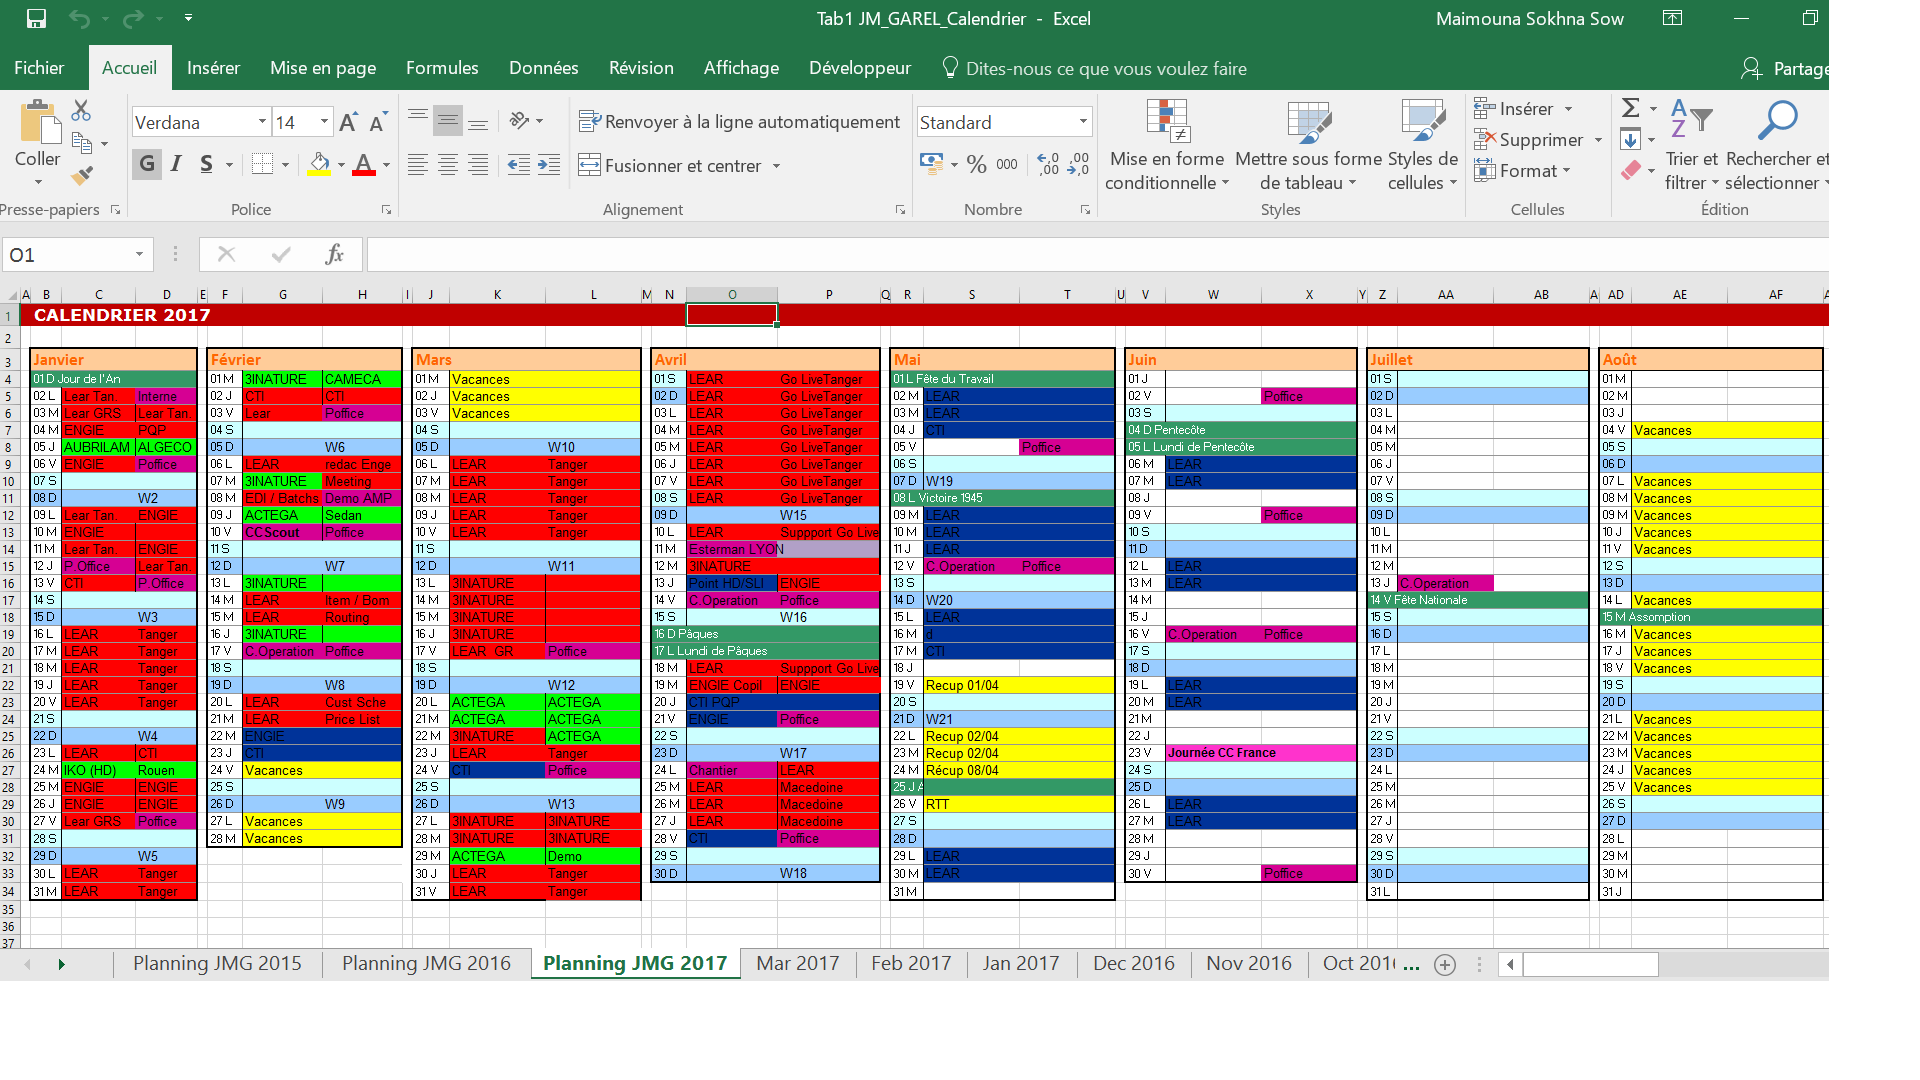
\includegraphics[scale=0.5]{images/annexe1.png}
\end{center}

\newpage
\textbf{Annexe 2}
\begin{center}
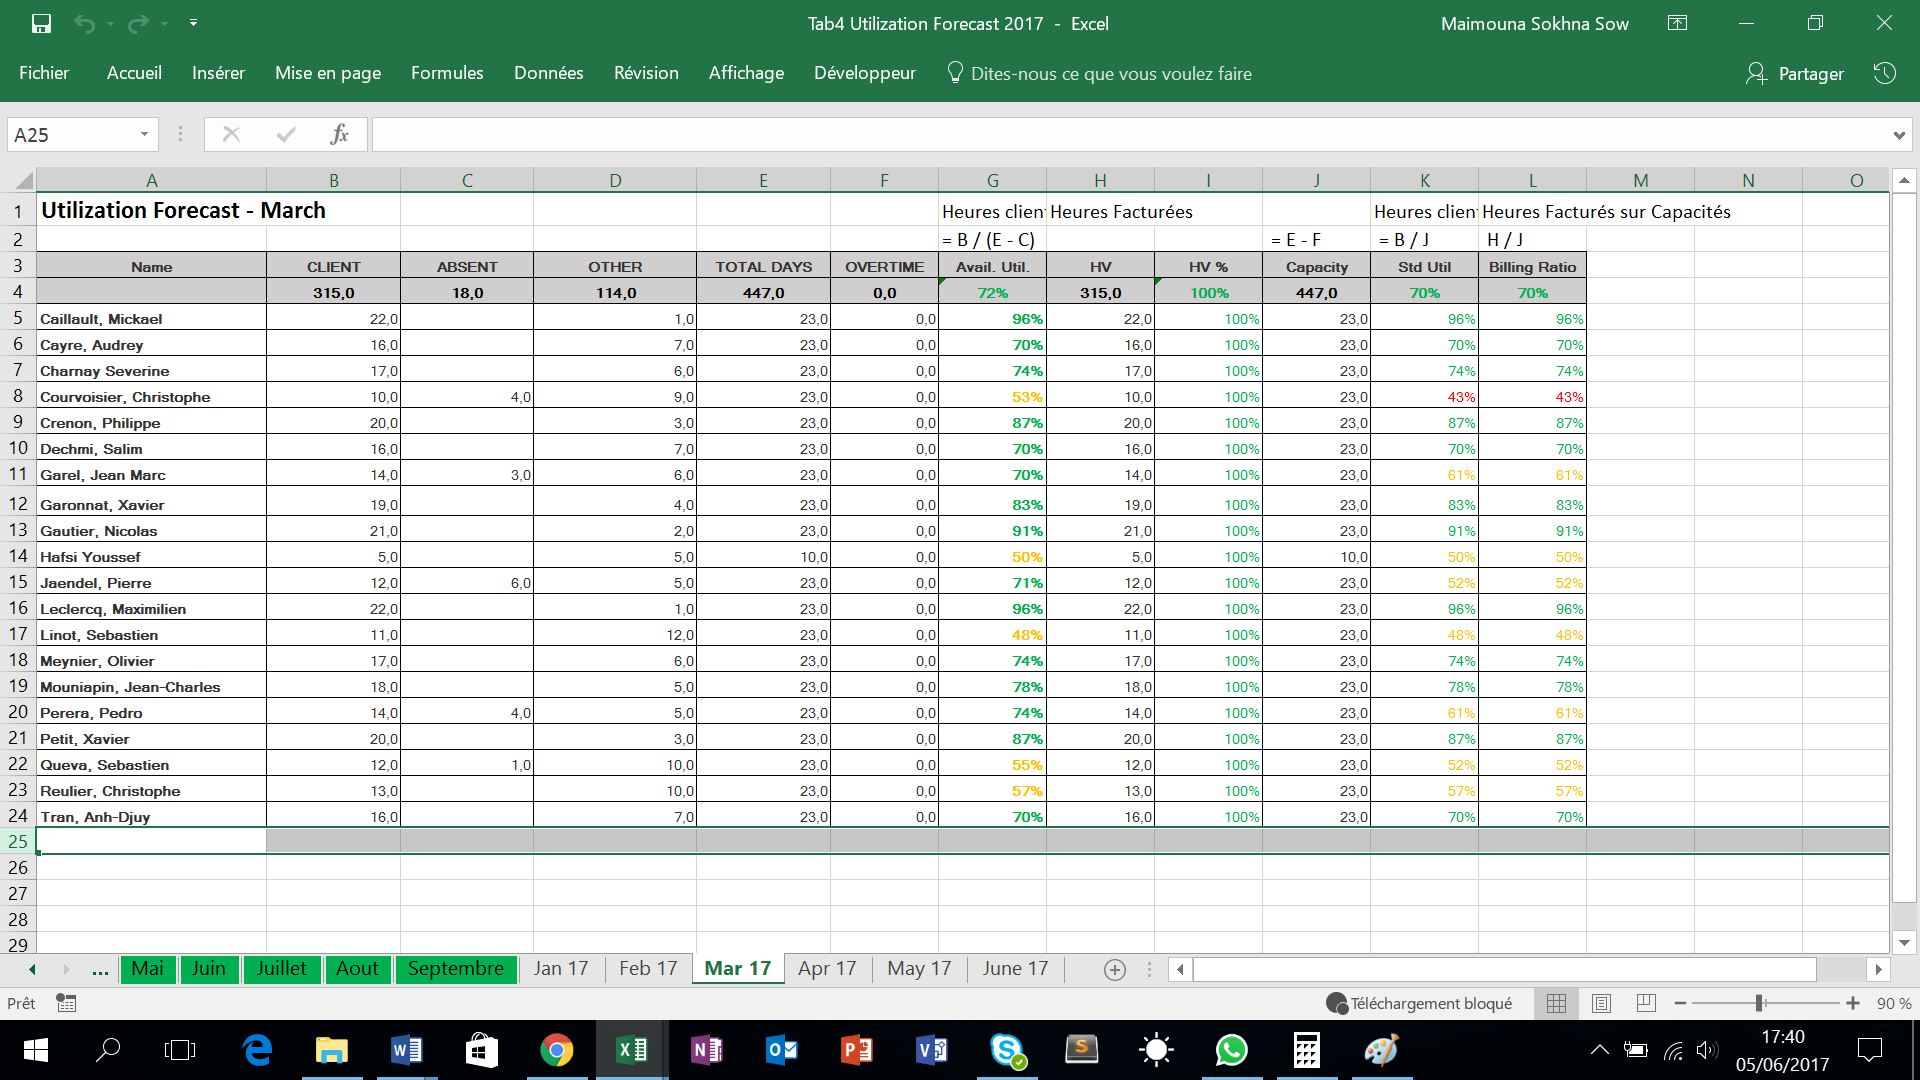
\includegraphics[scale=0.5]{images/annexe2.png}
\end{center}

\newpage
\textbf{Annexe 3}
\begin{center}
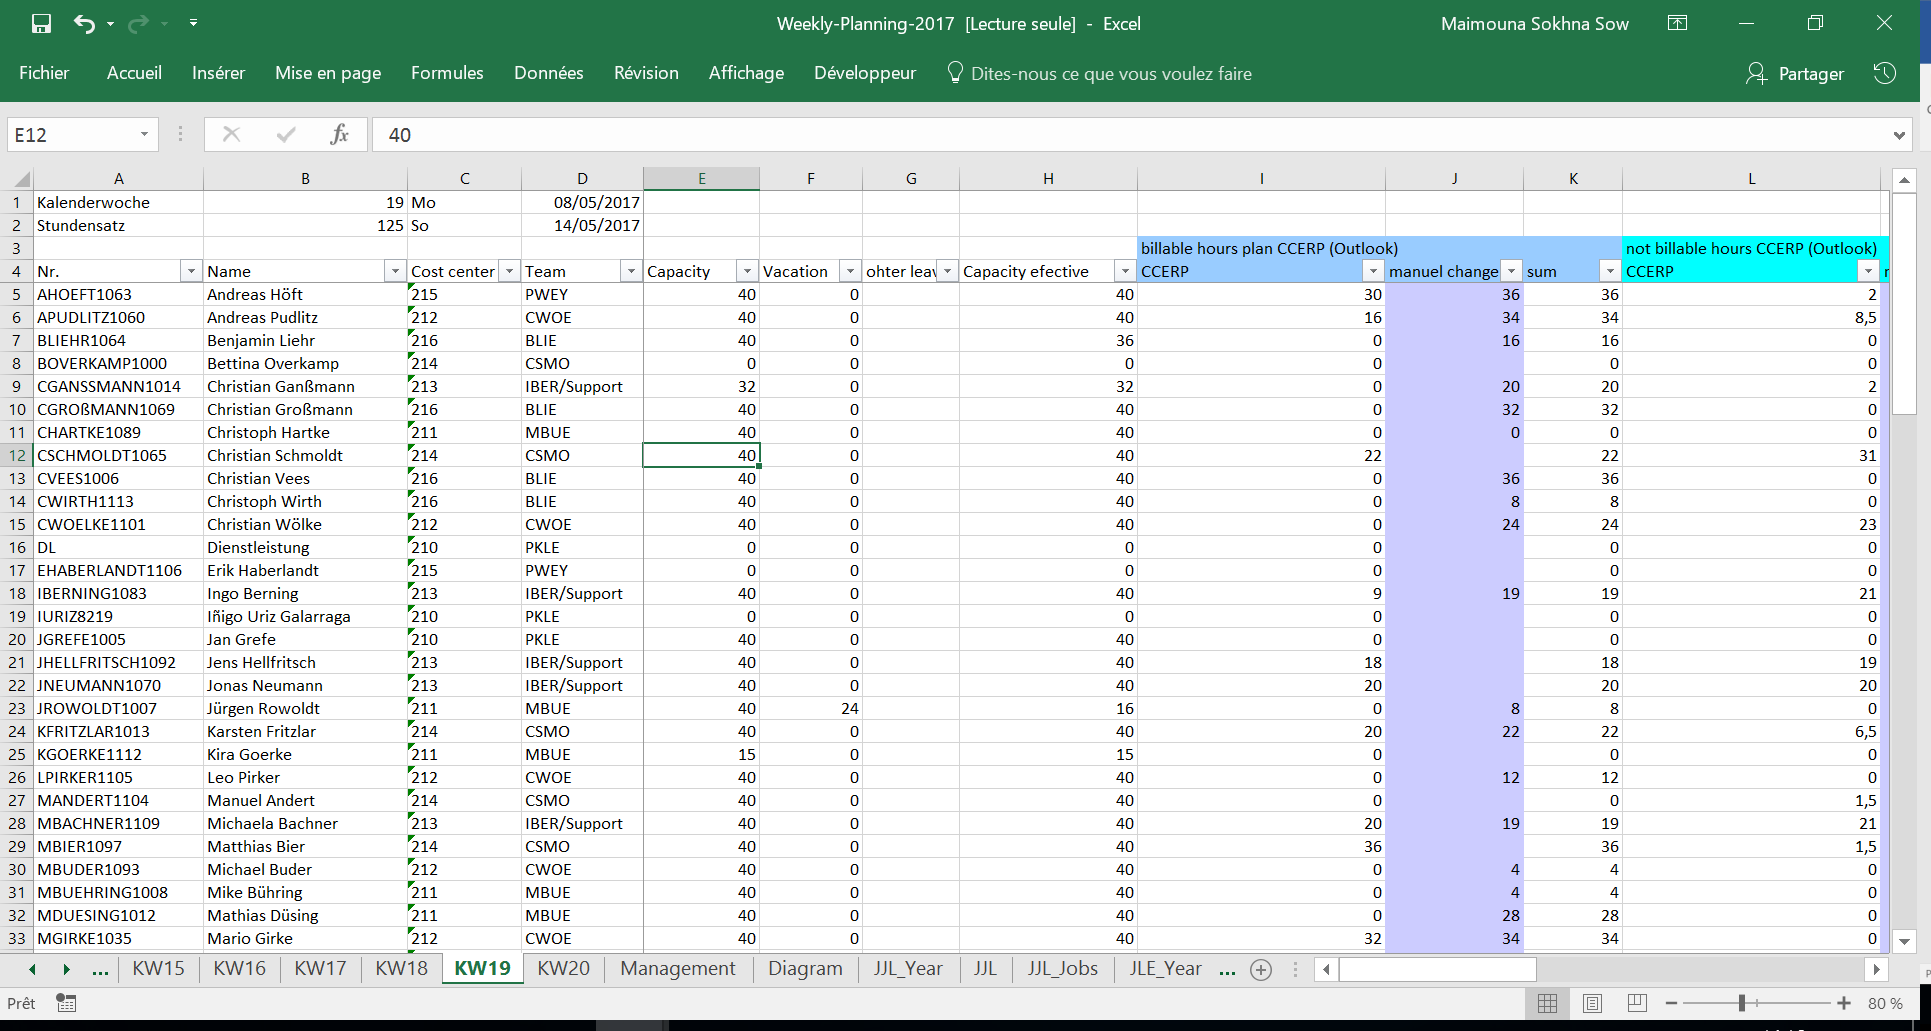
\includegraphics[scale=0.5]{images/annexe3.png}
\end{center}

\newpage
\section{Glossaire}
\begin{tabular}{|c|c|}
\hline 
\rowcolor{green}KEY & Value \\
\hline
ERP & Enterprise Resource Planning \\ 
\hline 
SI & Système d'Informations \\ 
\hline 
PME & Petites et moyennes entreprises  \\ 
\hline 
CC ERP & Cosmo Consult Enterprise Resource Planning \\ 
\hline 
QQOQCPC & Quoi Qui Où Quand Comment Pourquoi \\ 
\hline 
API & Application Programming Interface \\ 
\hline 
WBS & Work Breakdown Structure \\ 
\hline 
\end{tabular} 

\end{document}
